\documentclass[12pt,a4]{article}
\usepackage[a4paper, total={6.5in, 8.5in}]{geometry}
\usepackage{moreverb,url}
\usepackage[colorlinks,bookmarksopen,bookmarksnumbered,citecolor=red,urlcolor=red]{hyperref}
\usepackage{amssymb}
\usepackage{graphicx}
\usepackage[utf8]{inputenc}
\usepackage{amsmath}
\usepackage{pdfpages}
\usepackage{epstopdf}
\usepackage[english]{babel}
\usepackage{mathrsfs}
\usepackage{hyperref}
\usepackage{caption}
\usepackage{color}
\usepackage{float}
\usepackage[noabbrev]{cleveref}
\crefname{appsec}{appendix}{appendices}
\crefname{algocf}{algorithm}{algorithms}
\Crefname{algocf}{Algorithm}{Algorithms}
\usepackage{subcaption}
\usepackage{algorithm2e,algorithmic}
\usepackage{appendix}
%\usepackage{breqn}
\DeclareMathOperator{\sech}{sech}
\DeclareMathOperator*{\argmin}{arg\,min}

%
\bibliographystyle{elsarticle-num}

\begin{document}
%
\title{Motion planning of hyper-redundant robot through confined ducts}
%
%
\author{K. P. Ashwin*, Arkadeep N. C.
\thanks{Graduate Student at the Robotics and Design Lab, Department
of Mechanical Engineering, Indian Institute of Science, Bangalore 560012, India, email: ashwinkp@iisc.ac.in}, 
 and A. Ghosal
\thanks{Corresponding Author, Professor, Department of Mechanical Engineering, Indian Institute of Science, Bangalore, email: asitava@iisc.ac.in.}}
%
%double spacing for submission
%\baselineskip 12pt plus 0.5pt minus 0.5pt 
\baselineskip 18pt plus 0.5pt minus 0.5pt
%
\date{}
\maketitle
\begin{abstract}
\label{sec:abstract}
??
\end{abstract}

\textbf{Keywords}:??,??,??.
%\linenumbers

\section{Introduction}
\label{sec:introduction}
\begin{enumerate}
\item
\begin{itemize}
\item What are redundant robots
\item What is the use of redundancy
\item examples of applications of redundant robots
\item what is the downside?
\item what is called redundancy resolution. Say that the displacement of tip is specified and the co-ordinates(or the joint angles) of the subsequent links should be found out.
\end{itemize}

\item
\begin{itemize}
\item State that the major advantage of red. robots is obstacle avoidance
\item What is the first redundacy resolution scheme? Did it avoid obstacles?
\item How is obstacle avoidance included in red. resolution
\item Give a review of obstacle avoidance algorithms
\item state why tractrix is better, what is tractrix
\item how obstacle avoidance is easily implemented
\end{itemize}

\item
\begin{itemize}
\item State that particularly interesting is the case of motion through ducts, endoscopy and inspection
\item How the tractrix method as is is difficult to implement
\item Explain the motive of this paper
\item Contents of the paper
\end{itemize}
\end{enumerate}


\section{Overview of tractrix based motion planning}
\label{sec:Tractrixoverview}
%
Consider a rigid link of length $L_0$ positioned in a 2D plane, initially aligned to the Y-axis as shown in the figure[ref fig]. The co-ordinates of the `head' of the link is given as $\textbf{X}_h = [X_h,Y_h]^T$ and the co-ordinates of the `tail' as $\textbf{X}_t = [X_t,Y_t]^T$. If the head is displaced to the co-ordinate $\textbf{x}_h = [x_h,y_h]$ along the positive $X-$ axis by $t$ units, the tail of the link can lie anywhere on the circumference of a circle centered at the co-ordinate $(t,0)$ with radius $L_0$. If we assign a rule that the velocity of the tail of the link is always directed towards the length of the link, we get two diametrically opposite points on the circle. The continuous path traced by the tail point is the well known tractrix curve given by the expressions[ref]:
\begin{align}
\label{eq:tractrix}
\textbf{x}_t = [x(t),y(t)] = [t-L_0\tanh\frac{t}{L_0},L_0\sech\frac{t}{L_0}]
\end{align}
The extension of tractrix equation along motion in arbitrary direction as well as an algorithm to calculate the same in 3-D can be found in [ref] and [ref]. In case of multiple links connected to each other as in the case of hyper-redundant robot, or a one dimensional object approximated as a series of connected linkages the algorithm can be applied iteratively from the head to tail as shown in [ref]. By moving along the tractix curve, the tail moves the minimum distance with respect to its initial position. Also, the displacement $\Vert \textbf{x}_h-\textbf{X}_h \Vert \geq \Vert \textbf{x}_t-\textbf{X}_t \Vert$ which means that the displacement attentuates from the displaced link to end of the chain in case of serially connected links[fig2]. Due to the minimal displacement of the tail, the motion can be imagined as the one with high lateral resistance on the link and less resistance in the direction of motion of link. 

\begin{figure}[ht!]
    \centering
    \begin{subfigure}{0.48\textwidth}
        \centering
        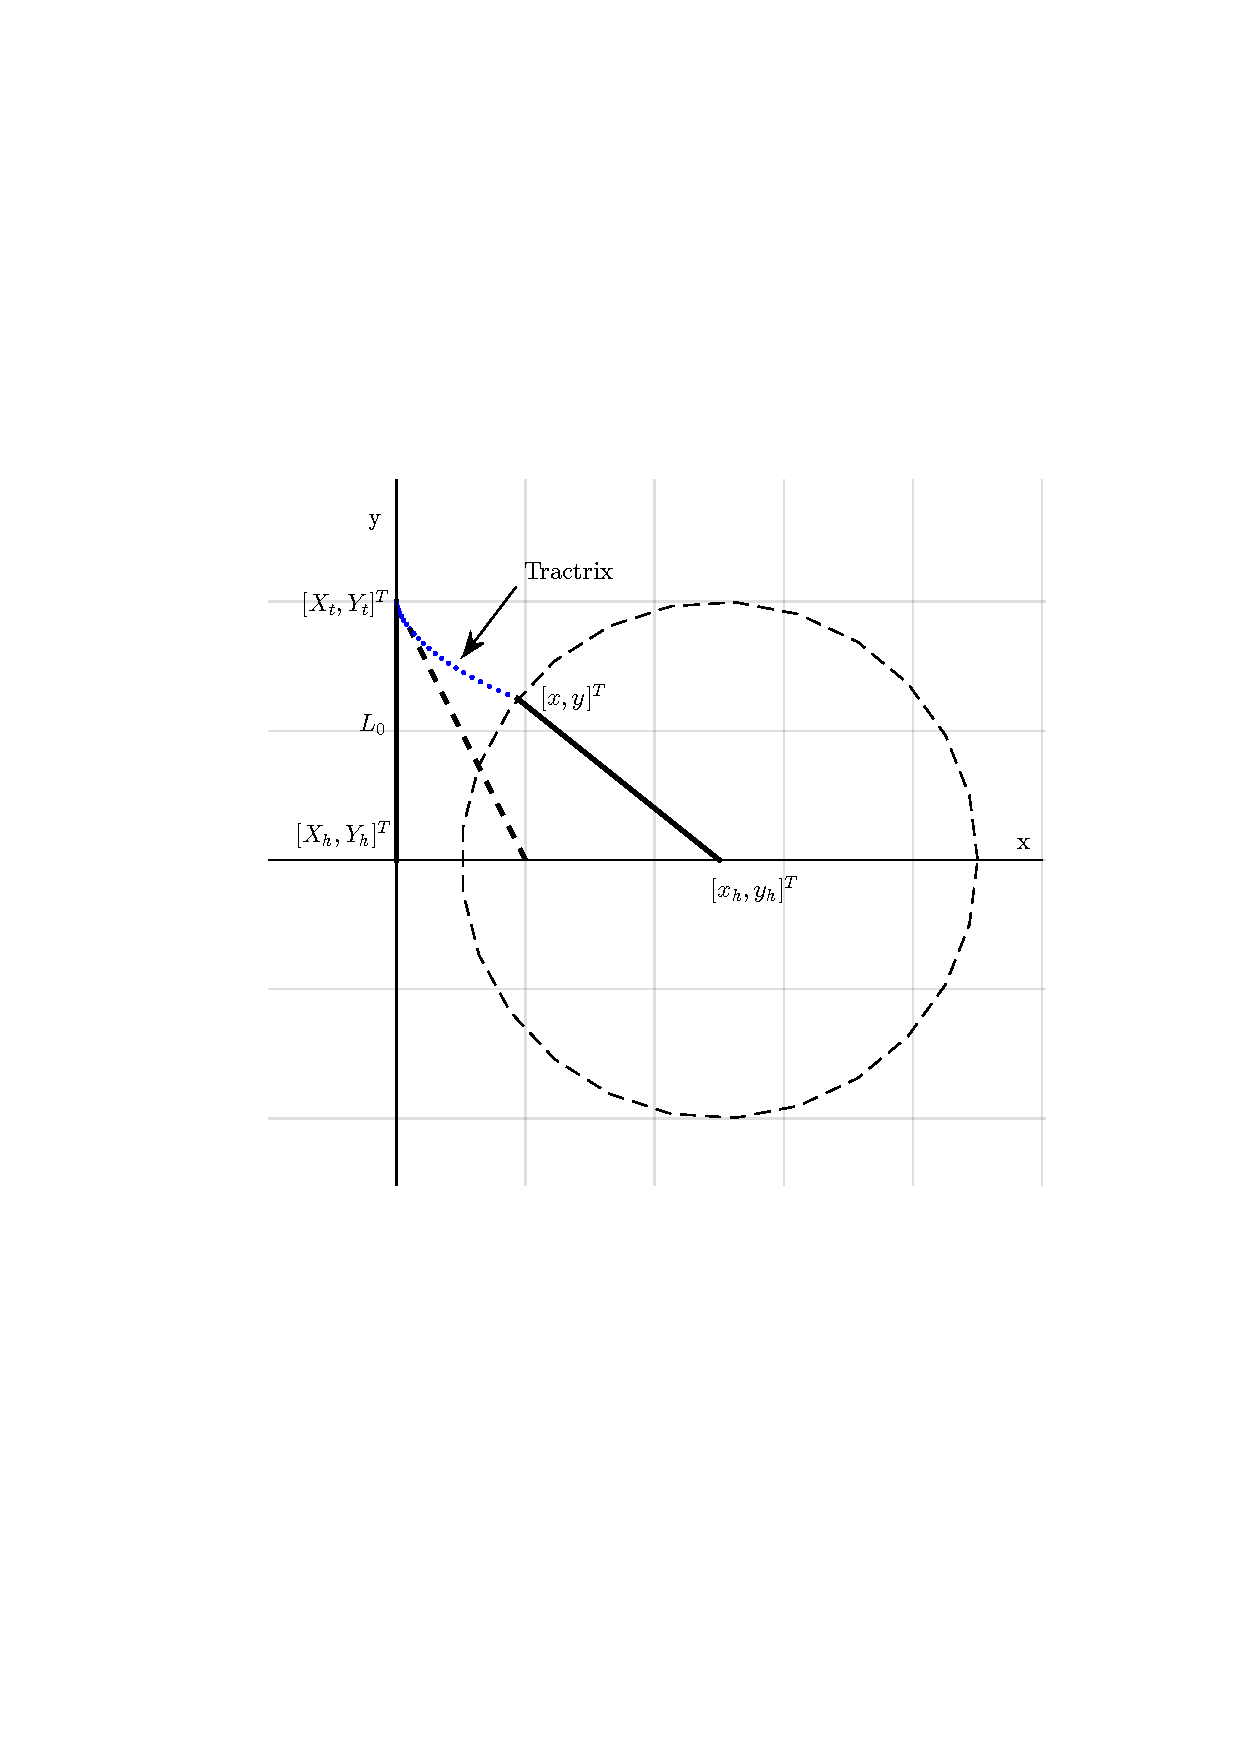
\includegraphics[width=\linewidth]{figures/fig1.pdf}
        \caption{Tractrix curve in 2D with one link}
        \label{fig:tractrixin2D}
    \end{subfigure}%
    \begin{subfigure}{0.48\textwidth}
        \centering
        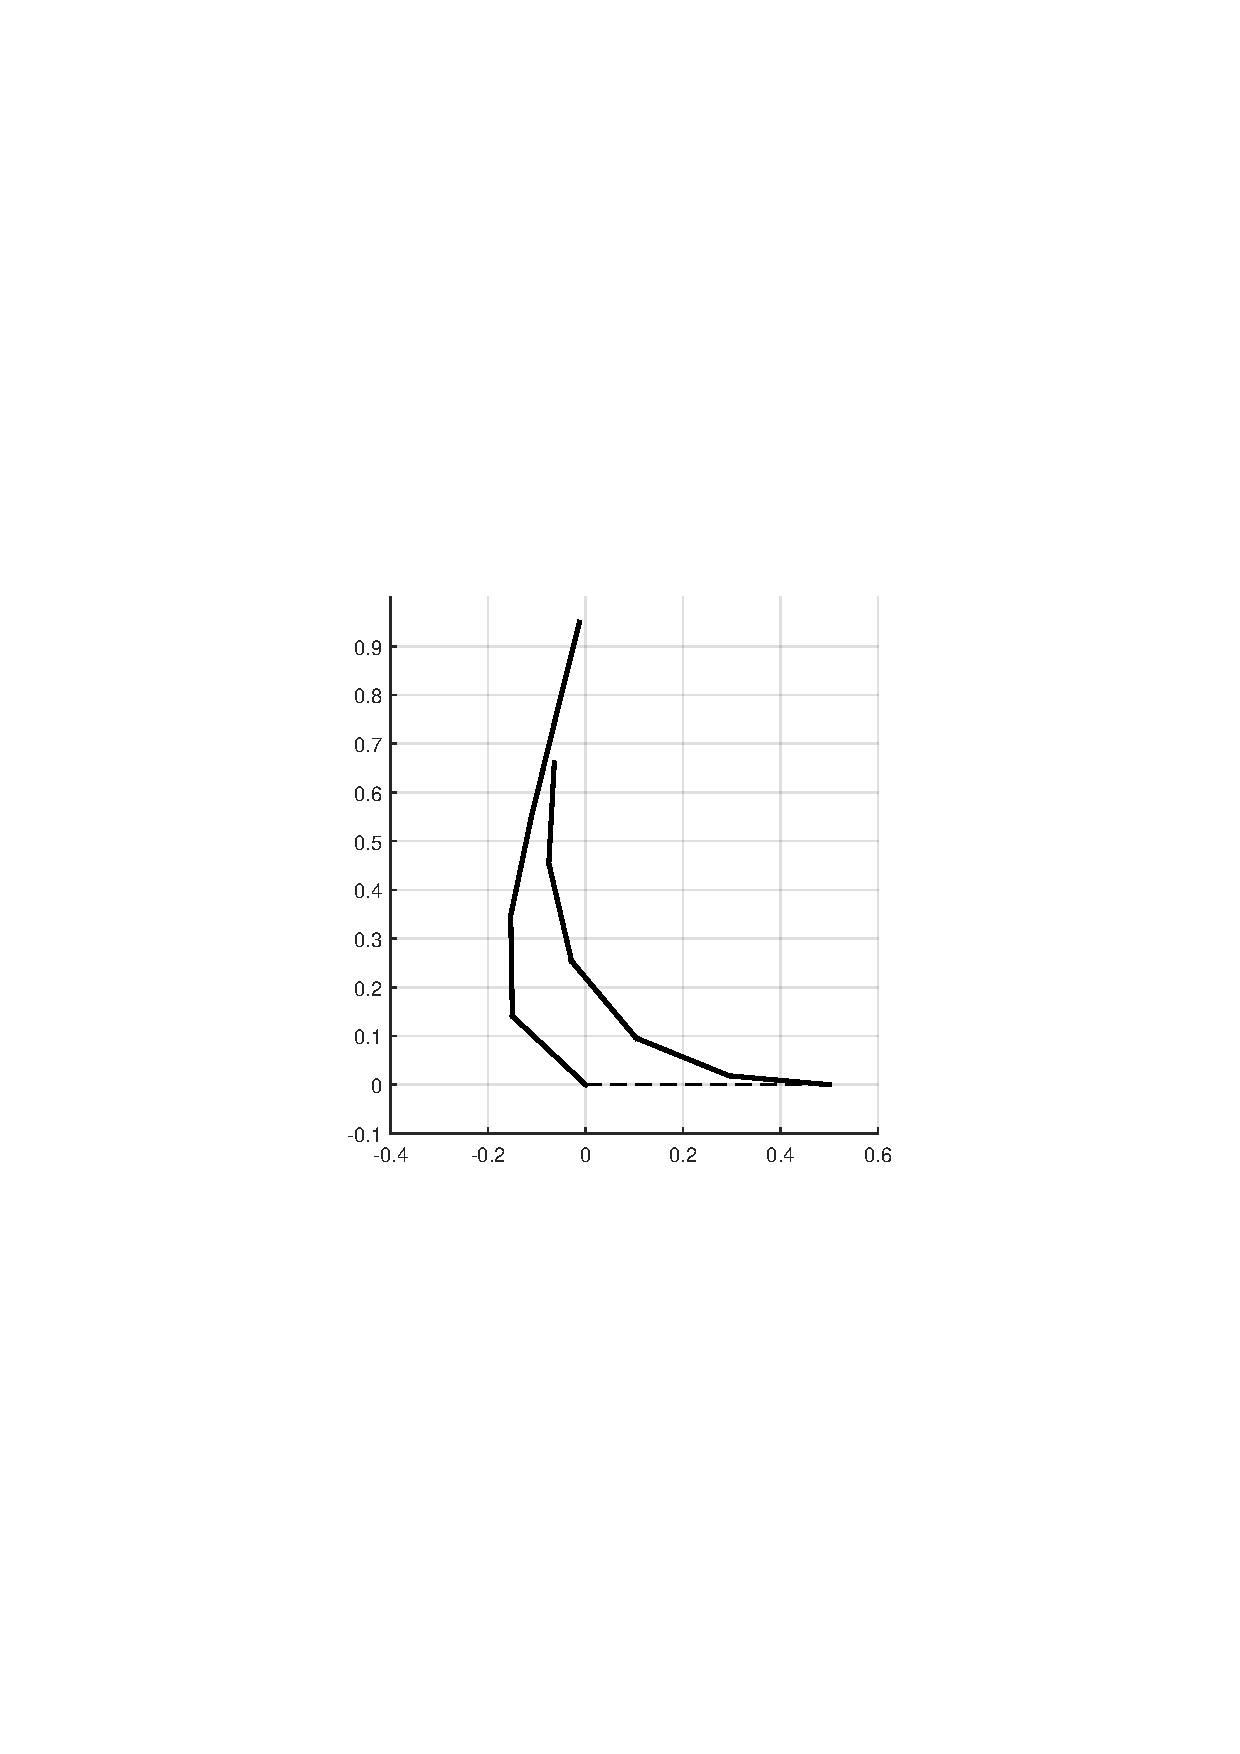
\includegraphics[width=0.75\linewidth]{figures/fig2.pdf}
        \caption{Tractrix with multiple links}
    \end{subfigure}
\caption{Tractrix in a plane}
\end{figure}


It is shown in [ref] that for a single rigid link, tractrix curve can also be obtained by minimizing an $L^2$ metric which is essentially the displacement of the tail from its initial position subject to the condition that the length of link is always preserved. i.e, the co-ordinates of the tail can be obtained from the following minimization problem:
\begin{align} \label{eq:Opt_prob_main}
\argmin_{\textbf{x}_t} &\Vert \textbf{x}_t-\textbf{X}_t \Vert\\
\text{Subject~ to:  } &\Vert \textbf{x}_h - \textbf{x}_t \Vert -L_0 = 0 \nonumber
\end{align}
An advantage of expressing tractrix as a minimization problem is that we can add more constraints to the above expression and hence, control the position of the tail point. Though the resulting curve may not necessarily be a tractix curve, the motion of the tail will appear realistic [ref]. For the motion of a link which minimizes its tail velocity (displacement of the tail co-ordinates), obstacle avoidance is achieved by formulating the problem as:
\begin{align} \label{eq:obstacle_avoidance_opt}
\argmin_{\textbf{x}_t} &\Vert \textbf{x}_t-\textbf{X}_t \Vert\\
\text{Subject to:} 
&\Vert \textbf{x}_h - \textbf{x}_t \Vert -L_0 = 0 \nonumber \\ 
~~ &f(\textbf{x}) \succeq 0  \nonumber
\end{align}
where $\bf{f}(x) = 0$ is the analytical equations of the boundaries of the surfaces which are to be avoided. For example, if the tail is to avoid a single obstacle represented by a circle with center $(x_c,y_c)$, the expression $f(x) = (x-x_c)^2+(y-y_c)^2-r^2>0$ ensures that the point $x$ always lies outside the circle of radius $r$. Complex objects can be modelled as a combination of super-ellipses as shown in [ref]. In this case, $f(x)$ will be a vector of all boundary equations $\textbf{f}(x) = [f_1(x),f_2(x),...f_m(x)]^T$ [fig3]. It is also worth noting that the value of function will increase or decrease as the point is farther from the curve $f(x)$; the value being zero on the curve. Hence, this approach can also be imagined as a geometric potential field, with zero potential only at the surface of the obstacle. 

\begin{figure}[h!]
\centering
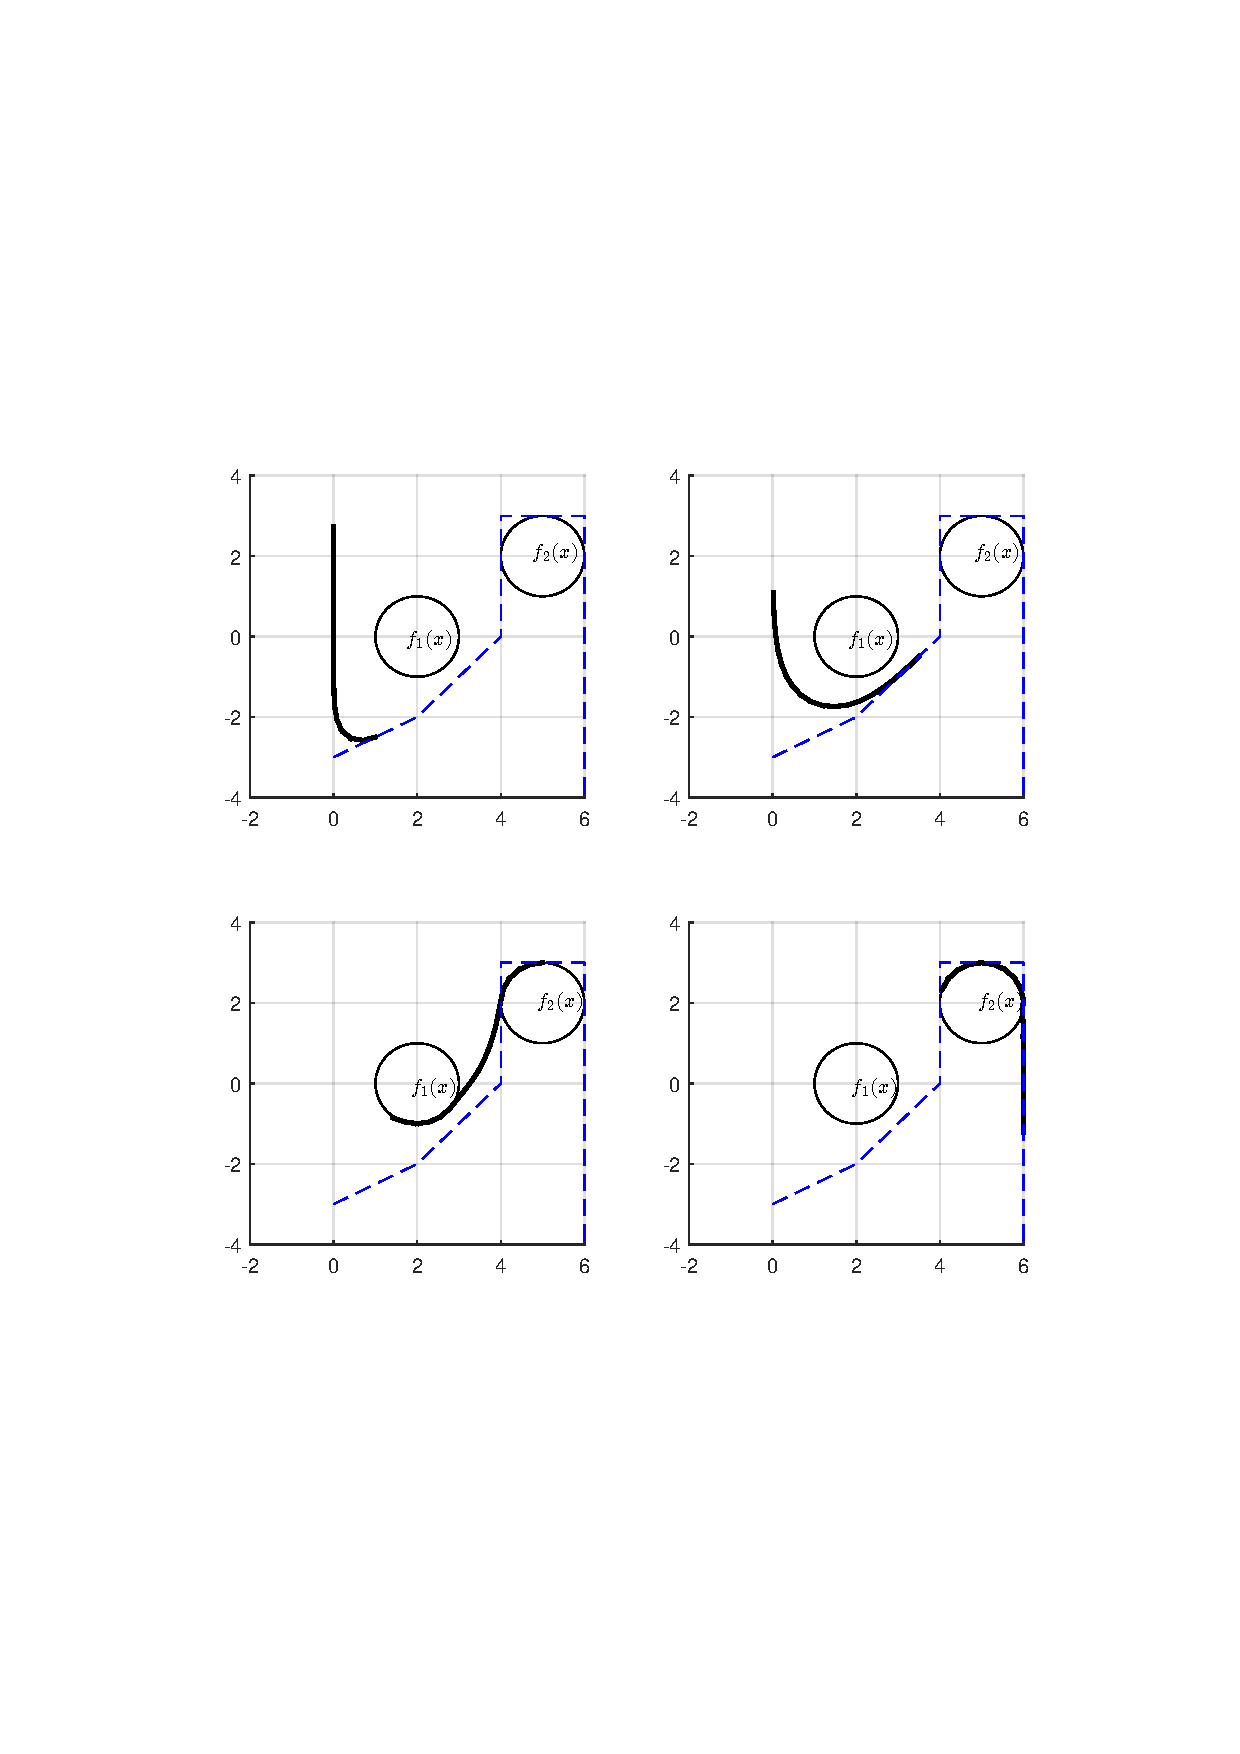
\includegraphics[scale=0.75]{figures/fig3.pdf}
\caption{Obstacle avoidance in a plane\label{fig:obstacle_avoidance_2D}}
\end{figure}

In the case of path planning of hyper-redundant manipulator, a majority of problems deal with simulating the motion of the robot while traversing through a confined space within a narrow bounded path, which we term as a ``\textit{duct}" for the remainder of the paper. The problem of planning the motion of the robot through a duct may be specified as:
\begin{align} \label{eq:path_planning_opt}
\argmin_{\textbf{x}_t} &\Vert \textbf{x}_t-\textbf{X}_t \Vert\\
\text{Subject to:} &\Vert \textbf{x}_h - \textbf{x}_t \Vert -L_0 = 0 \nonumber \\
<<<<<<< HEAD
 ~~ &{f}(x) <0 \nonumber
=======
 ~~ &{f}(x) \leq 0 \nonumber
>>>>>>> 1812e30da739acd007c5459920559282d36d3ae2
\end{align}
While this expression is applicable for a duct represented by a single surface with the boundary $f(x)$, unlike the obstacle avoidance problem, the same will not work in the case of complex surfaces represented by combination of simpler analytical shapes. This is because if a point is classified as inside one of the simpler shapes, then it should be classified as outside the other shapes forming the duct. In other words, if one constraint function $f_k(x)< 0$, then the other constraint functions $f_{i\neq k}\geq 0$. In the next sections, we present different methods to represent the ducts and how confined space motion is achieved in different cases. 


\subsection{Nature of the optimization problem}\label{sc:optimization}
In the previous section we have discussed how tractrix based motion planning can be formulated as a constrained optimization problem, which entails a discussion on the suitability of the posed optimization problem and guarantee that the solution is unique and physically tractable. To address this, we will prove that the problem in \cref{eq:path_planning_opt} and the variations of the same used in the current work can be posed as convex problems. A function $f:\mathbb{R}^n\to \mathbb{R}$ is \textit{convex} if and only if the following two conditions hold:
\begin{enumerate}
	\item [a] The domain of $f$, $\textbf{dom}f$ is a convex set, and,
	\item [b]  For all $x,y \in \textbf{dom}f$ and $\theta$ with $0\leq \theta \leq 1$ \begin{equation}\label{eq:convex_fn}
	f(\theta x+(1-\theta)y)\leq \theta f(x)+(1-\theta)f(y)
	\end{equation}
\end{enumerate}
In our problem, the function is the $L_2$ norm of a vector in $\mathbb{R}^2$ or $\mathbb{R}^3$.  Though the $L_2$ norm is defined for all real vectors, the constraints ensuring that the object moves within the confinement of the duct restricts the domain to a feasible closed set $\mathcal{S}$\footnote{Assuming $\mathcal{S}$ to be a closed set allows the object to physically touch the boundaries of the duct}. Therefore, if the conditions a and b associated with the definition of a convex function are satisfied for $\mathcal{S}$ and the $L_2$ norm, then the solution obtained for (put optimization equation here) is unique. \\ 
It is a well known result that any p-norm $||x||_p=(\sum\limits_{i=1}^{n}|x_i|^p)^{1/p},~ x\in \mathbb{R}$ is a convex function for $p\geq 1$. The fact that a p-norm is convex can be shown by using the scalability and the triangle inequality associated with a normed vector-space. With $\theta$  being a scaling parameter, \cref{eq:convex_fn} simplifies exactly to the triangle equality for norms. Also, any p-norm is a valid norm on $\mathbb{R}$ for $p\geq1$ follows from the Minkowski inequality\footnote{For a measure space $\mathbb{S}$, $p\geq 1$ and $f,~g$ are members of the Lebesgue space $L_P(\mathbb{S})$, the following inequality holds: $||f+g||_p\leq ||f||_p+||g||_p$ }. This leaves us to show that the feasible set $\mathcal{S}$ is convex. For all our modeling examples, we choose $\mathcal{S}$ to be convex by assigning convex boundaries to it or, expressing $\mathcal{S}$ as intersections of closed convex sets.  However, as is, none of the problems posed in \cref{eq:Opt_prob_main,eq:obstacle_avoidance_opt,eq:path_planning_opt} are convex because of the non-linear equality constraints associated with them, which guarantees that the length of a segment is constant. To pose it as a convex problem we approximate the constraint with 2 linear constraints as described in section(\textbf{put complexity section here}). For the cases of path planning in 2-D and 3-D, the paths chosen are either entirely convex or are discretized as such. As discussed in the following sections, we do not represent a ``duct" as a union of closed convex sets as the first condition of convexity cannot be guaranteed for sets formed by union of convex sets. 

\section{Motion planning through planar ducts}
%
In this section, we propose different methods to represent a duct in 2D planar surface. 
\subsection{Representation of duct using super-ellipses}
%
One method to represent a duct is by overlapping a series of super-ellipses as shown in [fig5b]. This is the most simple and straightforward means of representation as shown in [ref Midhun]. In Cartesian co-ordinate system $R^2$, the contour of super-ellipse obeys the following equation:
\begin{align}
f(\textbf{x})= f(x,y):\quad \left \vert \frac{x-x_c}{a} \right\vert^n+\left\vert \frac{y-y_c}{b} \right\vert^n-1=0
\end{align}

\begin{figure}[h]
\centering
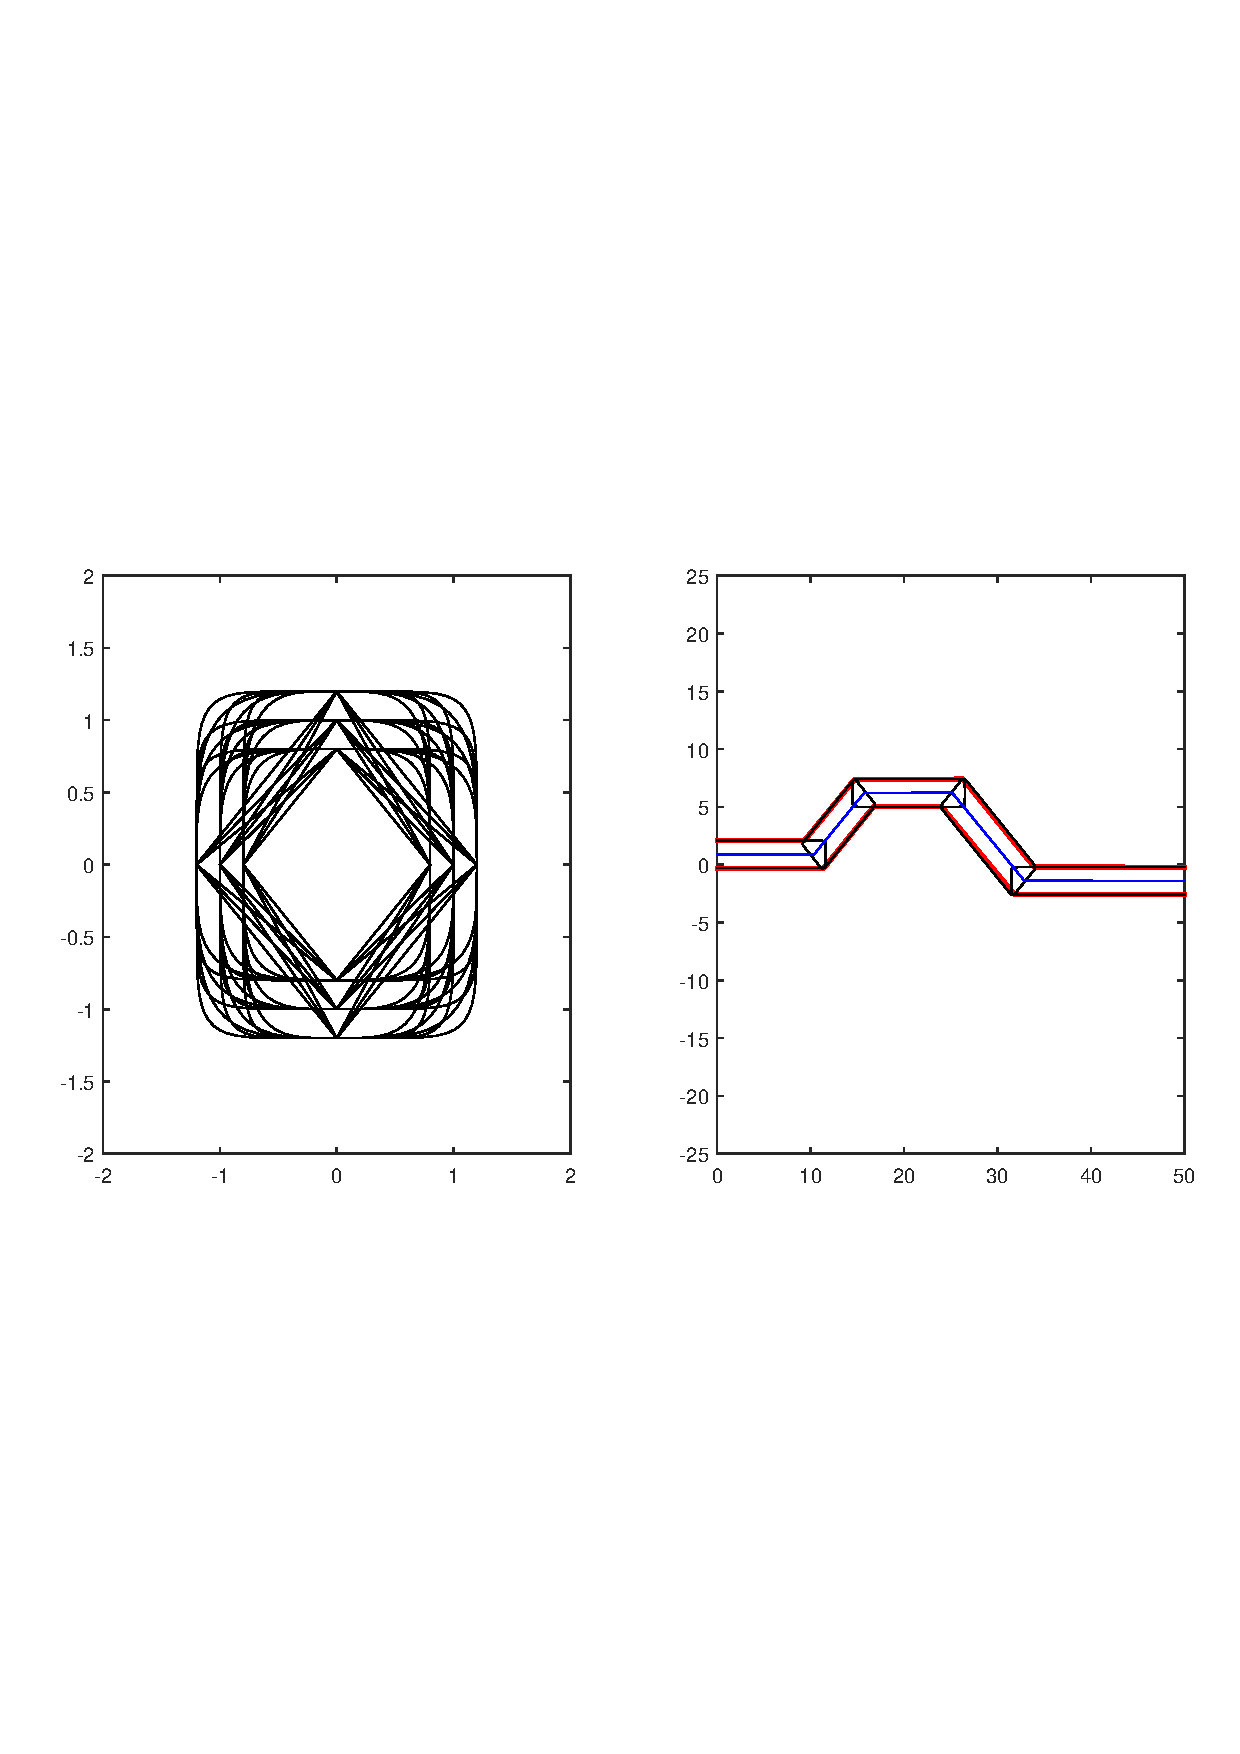
\includegraphics[scale=0.75]{figures/fig4.pdf}
\caption{ Super-ellipses and a duct modelled as combination of super-ellipses\label{fig:super-ellipses}}
\end{figure}

The condition $f(\textbf{x}_t)<0$ will ensure that the co-ordinates of the tail of the link $(x_t,y_t)$ always lie inside the bounding curve of a super-ellipse. However, in case of multiple equations (${f_i(x)},~ i=1,2,...,m$), only one of them will be satisfied for the point to be inside the duct. In practical implementation, we can say that this translates to saying that the least value amongst all the values of ${f_i(x)}$ should be less than zero. For the $i^\text{th}$ super-ellipse which is rotated by an angle $\phi_i$ about the $z-$ axis and whose center is translated to the co-ordinates $(x_i,y_i)$ so as to fit a portion of a duct, the co-ordinates of boundary should be multiplied with a transformation matrix
\begin{align}
T_i = \begin{bmatrix}
\cos \phi_i & -\sin\phi_i & 0 & x_i\\
\sin \phi_i & \cos\phi_i & 0 & y_i\\
0 & 0 & 1 &0\\
0 & 0 & 0 & 1
\end{bmatrix}
\end{align}
The constraint equation now becomes $g_i(\textbf{x}_t) : f_i(T_i^T\textbf{x}_t)< 0,~ i=1,2,...,m$ and, the complete formulation is given as:
\begin{align}
\label{eq: min_and_mingx}
\argmin_{\textbf{x}_t} &\Vert \textbf{x}_t-\textbf{X}_t \Vert\\
\text{Subject ~to:~~~} &\Vert \textbf{x}_h - \textbf{x}_t \Vert -L_0 = 0 \nonumber \\
& \min\left(g_i(\textbf{x}_t)\right) < 0, i=1,2,...,m \nonumber
\end{align}

An example of single link and multi-segmented chain passing through the duct is shown in [fig5]. Motion of a unit link with and without constraint is shown in [fig6]. The negative gradient (descend direction) of the inequality constraint function is also shown in the figure. The method shown here is quite fast and scalable as explained in section ??, while the majority of time taken for the scheme being in identifying the super-ellipsoids which fit the duct profile. For the example shown in this section, this identification is done by manually selecting clusters of points in the duct and fitting ellipses which will reduce the fitting error in a least squared sense.

\begin{figure}[h]
\centering
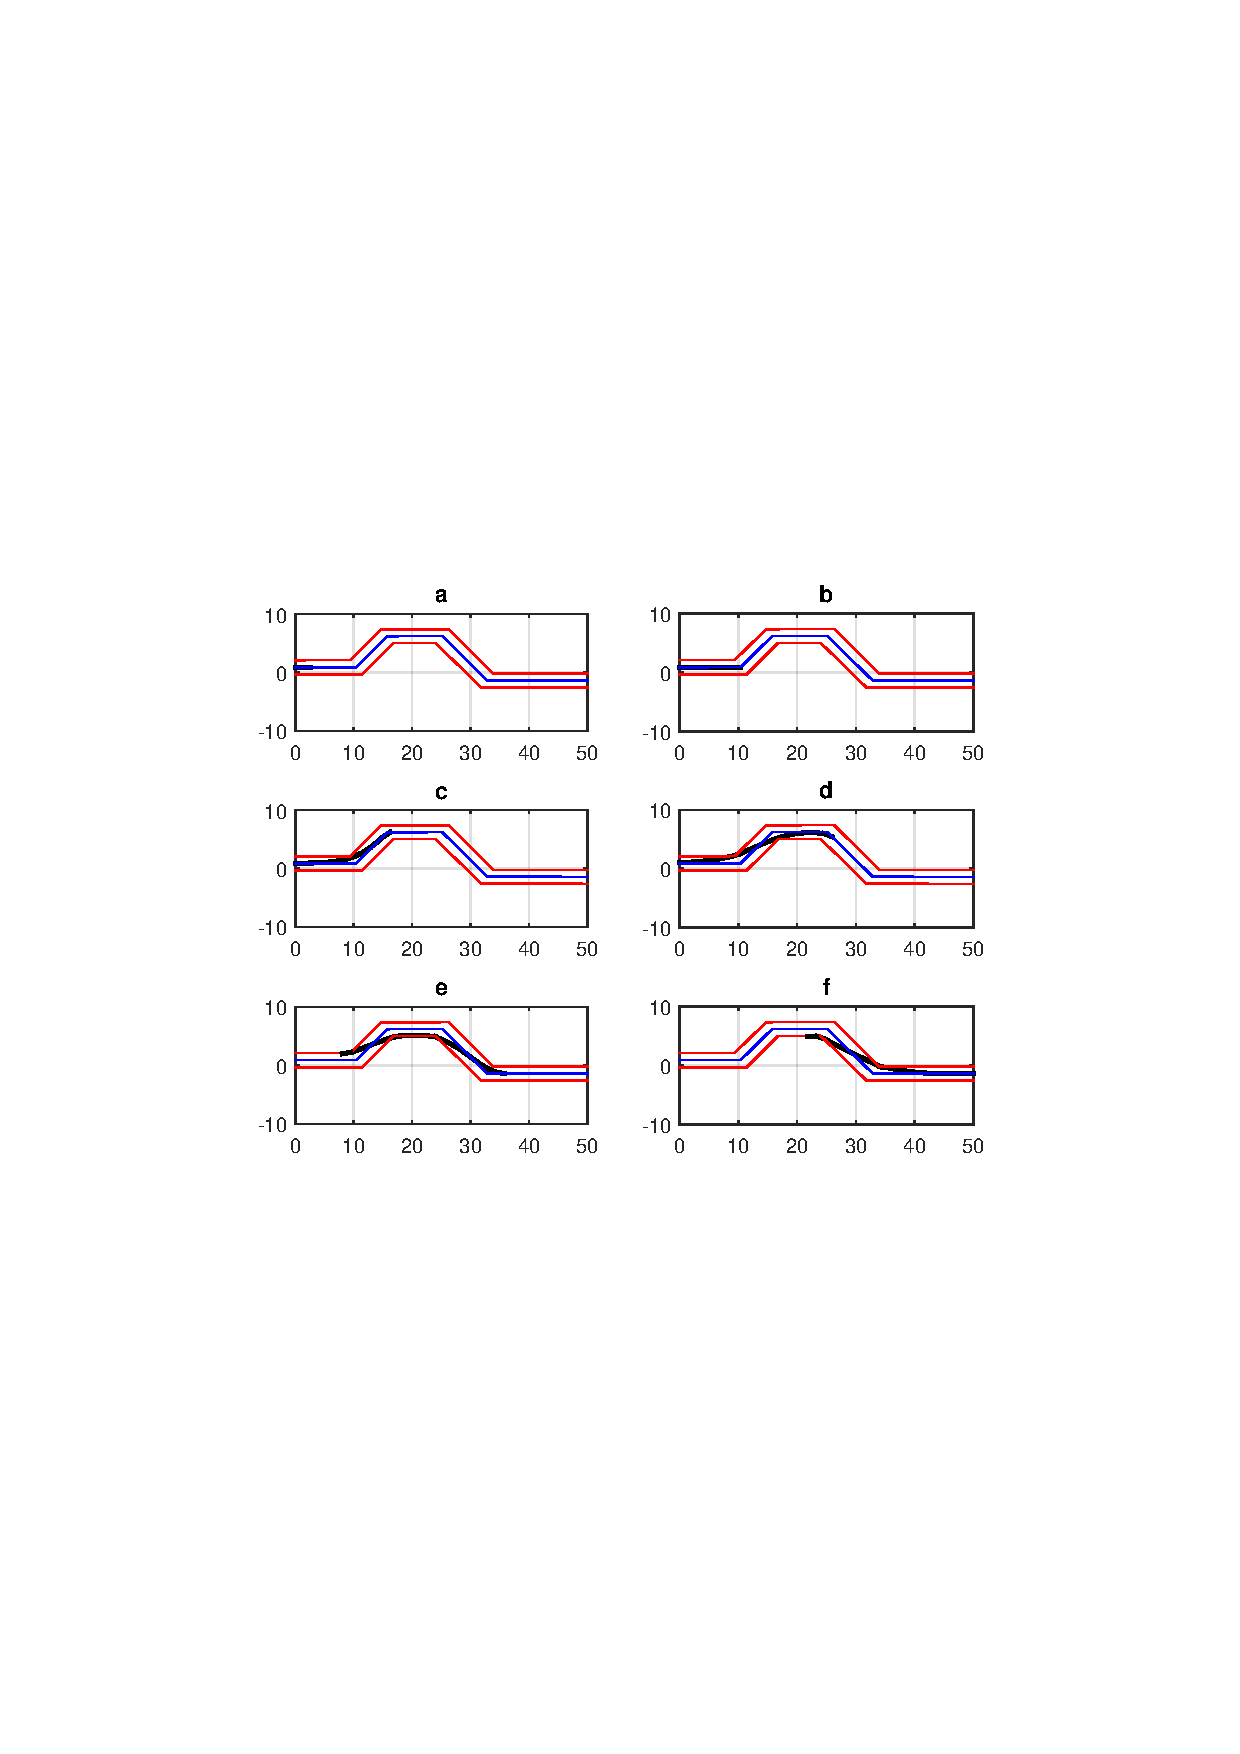
\includegraphics[scale=0.5]{figures/fig5.pdf}
\caption{ Motion through duct modelled as combination of super-ellipses\label{fig:ductasSEs}}
\end{figure}

\begin{figure}[h]
\centering
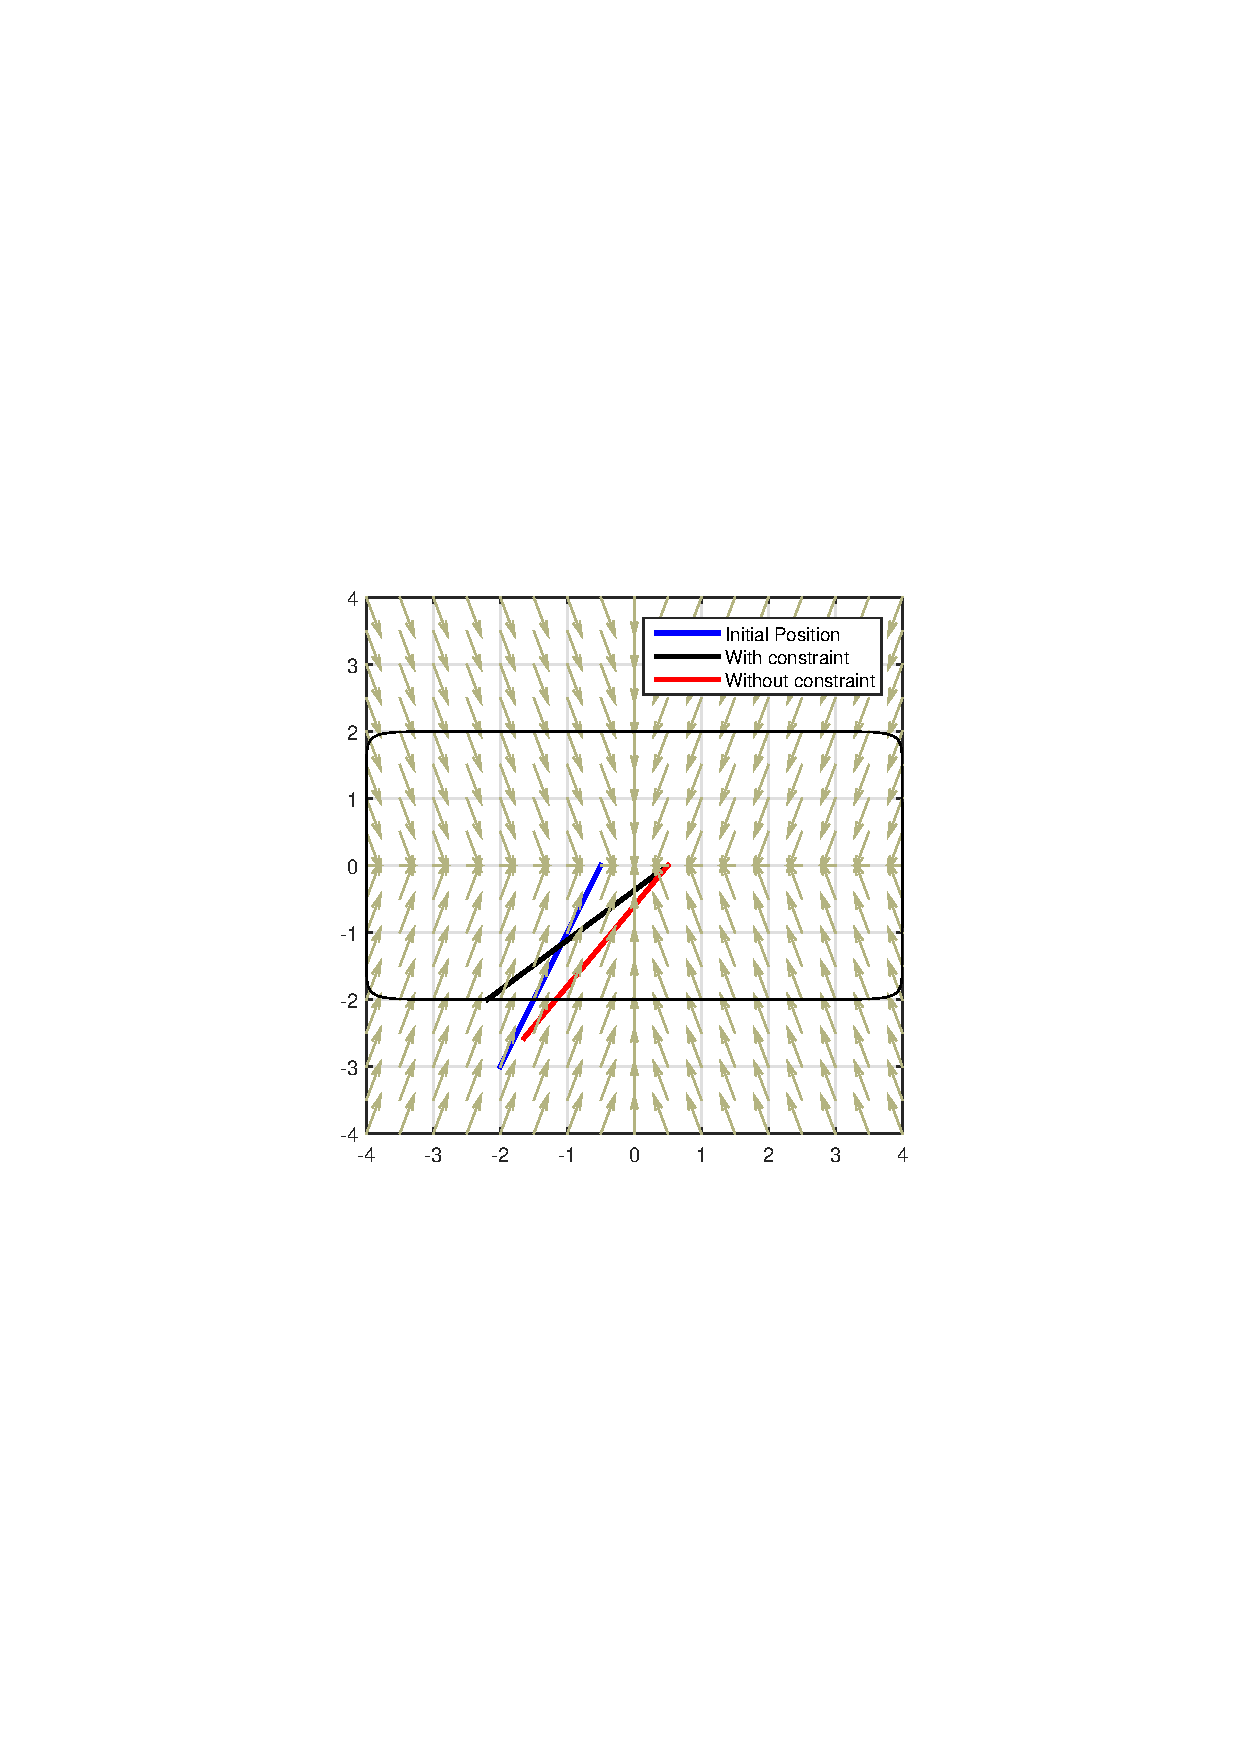
\includegraphics[scale=0.5]{figures/fig6.pdf}
\caption{ Effect of gradient of inequality constraint in pulling the tail into the duct\label{fig:gradienteffectSE}}
\end{figure}


\subsection{Representation of duct as a set of connected quadrilaterals}

Since the profile of a super-ellipse is always symmetric, for complex and non-symmetric ducts, representation using the previous method might require a large number of shapes. In such cases, a complex duct shape can be represented as a continuous array of discrete patches formed by piecewise continuous curves as shown in [fig6]. The individual quadrilateral patches may be denoted as $A_1,A_2,...,A_n$, each bounded by the line segments defined by the points $\mathbf{(P_0,P_1),(P_1,P_2),...,(P_{n-1},P_n)}$ for the curve $\mathbf{\zeta_1}$ and $\mathbf{(Q_0,Q_1),(Q_1,Q_2),...,(Q_{n-1},Q_n)}$ for the curve $\mathbf{\zeta_2}$. Then the co-ordinates of a point inside the surface patch $A_i$ is given by the parametric expression
\begin{align}
\label{eq:xi(u,t)}
\mathbf{x}_i(u,v)= \left[ \mathbf{P}_{i-1}+\left(1-{u} \right)\mathbf{P}_i  \right]\left(1-{v}\right) +\left[\mathbf{ Q}_{i-1}+\left(1-{u} \right)\mathbf{Q}_i  \right]\left({v}\right)
\end{align}
in parameters $u$ and $v$. If the vertices of the quadrilateral are given by $\mathbf{P}_{i}=\left[ {}^xP_{i},{}^yP_{i}\right]^T $ and $\mathbf{Q}_{i}=\left[ {}^xQ_{i},{}^yQ_{i}\right]^T $, then the analytical expressions for the terms $u$ and ${v}$, given the value of $\mathbf{x}_i$, can be obtained by solving \ref{eq:xi(u,t)} (see Appendix). The values of $u,v$ can be used to classify the point with respect to the surface patch $A_i$\footnote{It may be noted that there will be two sets of solution and they are not always real and unique. For example, the point $\mathbf{P} =\left(10,-5 \right)$ when classified with respect to the area $A$ given by the points $\mathbf{P}_1 = \left(0,15 \right),\mathbf{P}_2 = \left(10,10 \right),\mathbf{Q}_1 = \left(0,0 \right)$ and $\mathbf{Q}_2 = \left(4,1 \right),$ returns the values $u=\left( 1.0 + 0.6~i,~1.0 - 0.6~i \right)$ and $v=\left(2.0 + 1.9~i,~2.0 - 1.9~i\right)$. However, it is a trivial task to filter out the imaginary set of solutions, should the algorithm encounters the same.}.

\begin{figure}[h]
\centering
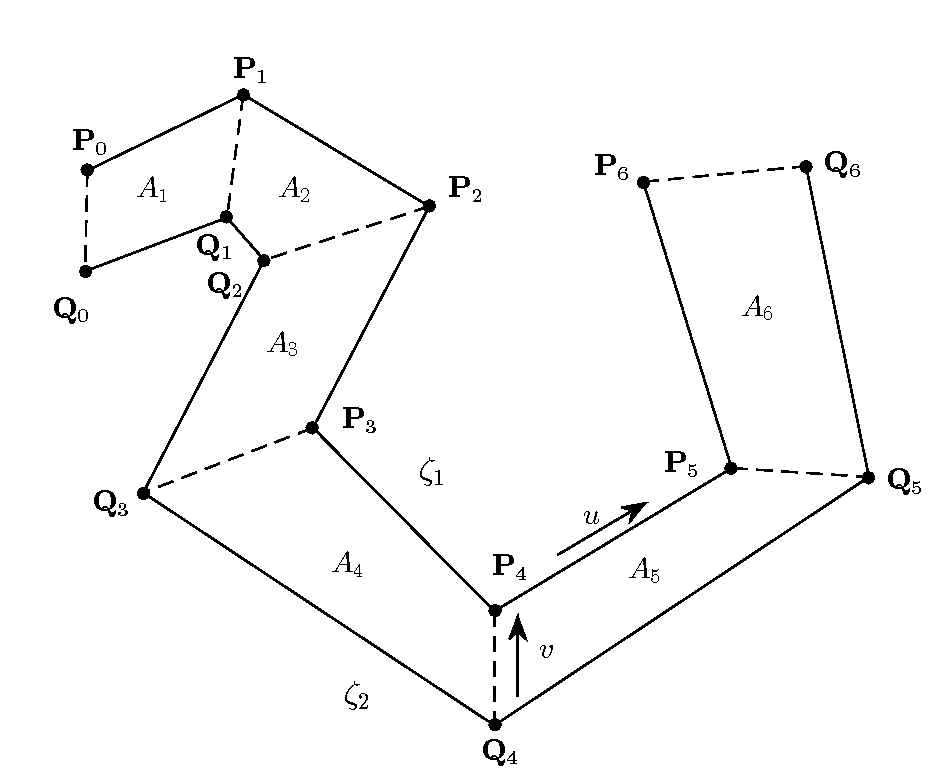
\includegraphics[scale=0.5]{figures/fig7.pdf}
\caption{Duct represented by stitched quadrilaterals\label{fig:stitchequads}}
\end{figure}

 In case of a single quadrilateral patch, we can now write the optimization problem as:
 \begin{align}
 \label{eq:minx,u,v}
\min_{\textbf{x}_t} &\Vert \textbf{x}_t-\textbf{X}_t \Vert\\
\text{Subject to:~~~} &\Vert \textbf{x}_h - \textbf{x}_t \Vert -L_0 = 0\\
\text{~~~~~~~} 0 \leq &u \leq 1\\
\text{~~~~~~~} 0 \leq &v \leq 1
\end{align}
for real values of ${u}$ and ${v}$. In case of multiple patches, classifying one point with respect to all the patches return the values $\left({u}_1,{v}_1 \right), \left({u}_2,{v}_2 \right),...,\left({u}_m,{v}_m \right)$ etc. for the $m$ number of patches $A_1, A_2,..., A_m$ and consequently, $m$ set of conditions. But out of the $m$ condition sets, only one set should be satisfied since the point will belong to only one patch at a given instance of motion through the duct. Including a switching  statement in the optimization code will be inefficient especially when the point to be classified is close to the common boundary between two patches. 

In order to provide a gradient to the constraint which will direct the point into the duct, an inequality constraint is to be included as in the case of super-ellipses described in the previous subsection. If $\hat{u}$ and $\hat{v}$ represent the parameters obtained for a point $\mathbf{x}_t$ classified with respect to the quadrilateral $A_i$, $x_{\zeta_1}(t) = \mathbf{P}_{i-1}+\left(1-{\hat{u}} \right)\mathbf{P}_i$ and $x_{\zeta_2}(t) = \mathbf{Q}_{i-1}+\left(1-{\hat{u}} \right)\mathbf{Q}_i$ will give the two points on the duct boundary curves corresponding to the parameter $\hat{u}$. Then using triangular inequality theorem ??, we can see that the value
\begin{align}
\label{eq:ductgradientinquad}
h = \Vert \mathbf{x}_{\zeta_1}-\mathbf{x}_t\Vert^2+\Vert \mathbf{x}_{\zeta_2}-\mathbf{x}_t\Vert^2-\Vert \mathbf{x}_{\zeta_1}- \mathbf{x}_{\zeta_2}\Vert^2
\end{align}
will always assign a negative real value for $h$ when point is inside the duct and a positive real value when the point is outside the duct. The value will be zero only at the boundaries. Hence, for an array of quadrilaterals, it is only necessary that the minimum value of the vector $\mathbf{h} = [{h}_1, {h}_2,...,{h}_m]$ should be negative for classifying the point with respect to the duct, as in the case of previous section. But as we can see, the inequality only takes into account the parameter variation across the boundaries (along the parameter $v$) and not in the direction of $u$ which could result in erroneous classification. For example, with reference to the figure [fig 9b], the value of $h$ for the point $\mathbf{P}$ classified with respect to the two quadrilaterals are $h_1 = ??$ and $h_2 = ??$. Hence, a minimum of both the values will wrongly classify the point as inside. To account for the same, we make use of the function $\chi$ which is necessarily a linear combination of two Heaviside step functions $H(0)-H(1)$, defined as:

\begin{align}
\label{eq:chifunction}
\chi(t) = \left\lbrace \begin{matrix}
0,&\quad t<0 \\
1,&\quad 0\leq t \leq 1\\
0, &\quad t >1
\end{matrix}\right.
\end{align}
The function $\chi$ applied on the quantity $\hat{u}_i$ (which is the value of parameter ${u}$ classified with respect to quadrilateral $A_i$), will return 0 only if the point satisfies the constraint $0\leq \hat{u}_i\leq 1$. Now, multiplying this quantity $\chi(\hat{u})$ with $h_i$ will return a non-zero negative value only if the point is inside the duct. Including the inequality constraint, the complete optimization problem is given as:

\begin{align}
\label{eq:min,u,v,im}
\min_{\textbf{x}_t} &\Vert \textbf{x}_t-\textbf{X}_t \Vert\\
\nonumber \text{sub:~~~} &\Vert \textbf{x}_h - \textbf{x}_t \Vert -L_0 = 0\\
&\left[\chi\left(\hat{\mathbf{u}}\right)\right]^T\mathbf{h}<0
\end{align}
where $\hat{\mathbf{u}}=\left[\hat{u}_1,\hat{u}_2,...,\hat{u}_m\right]^T$

Motion of a unit link passing through the duct is shown in [fig11] and the effect of the added inequality constraint to pull the tail end of the link which is initially positioned outside the duct, is shown in [fig12]

\begin{figure}[h]
\centering
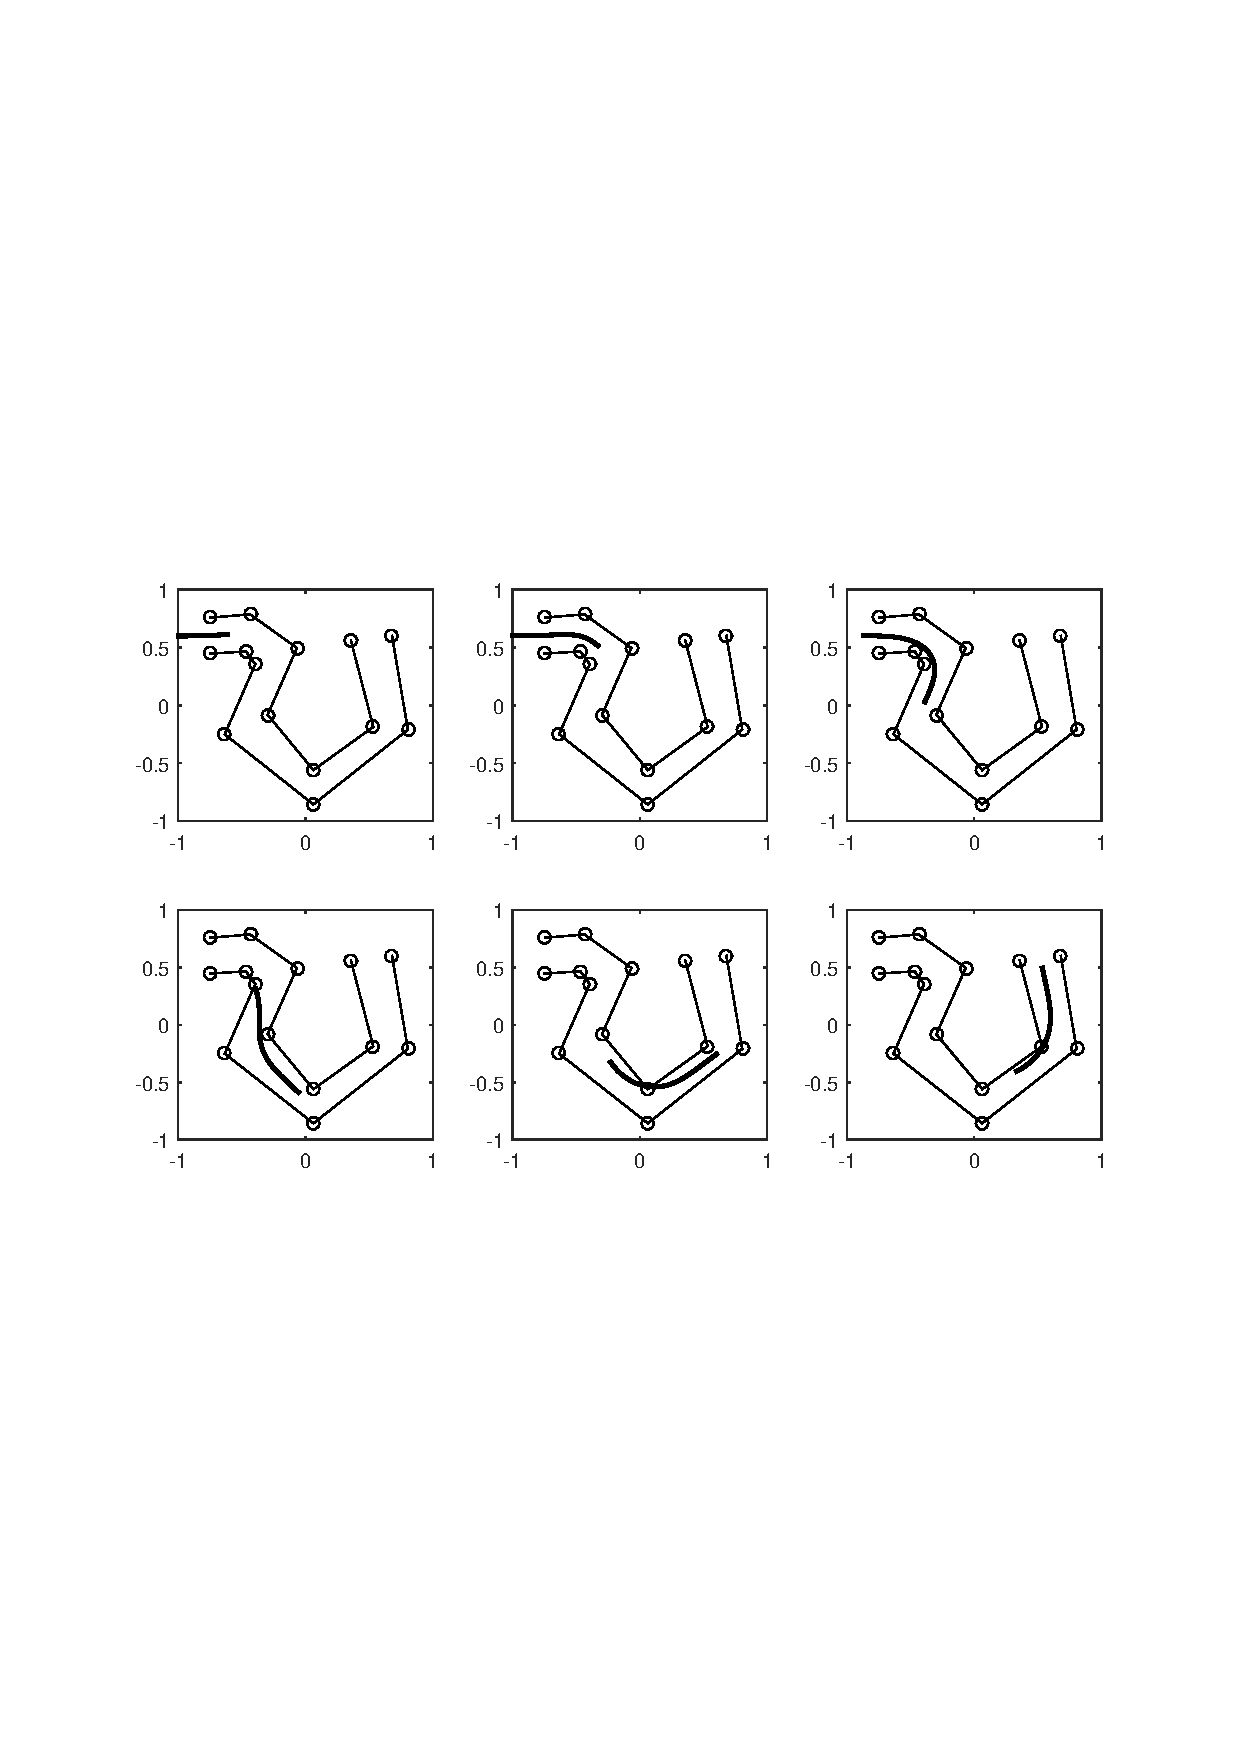
\includegraphics[scale=0.75]{figures/fig10.pdf}
\caption{ Example of constrained motion with stitched quadrilaterals \label{fig:motionquads}}
\end{figure}

\begin{figure}[h!]
\centering
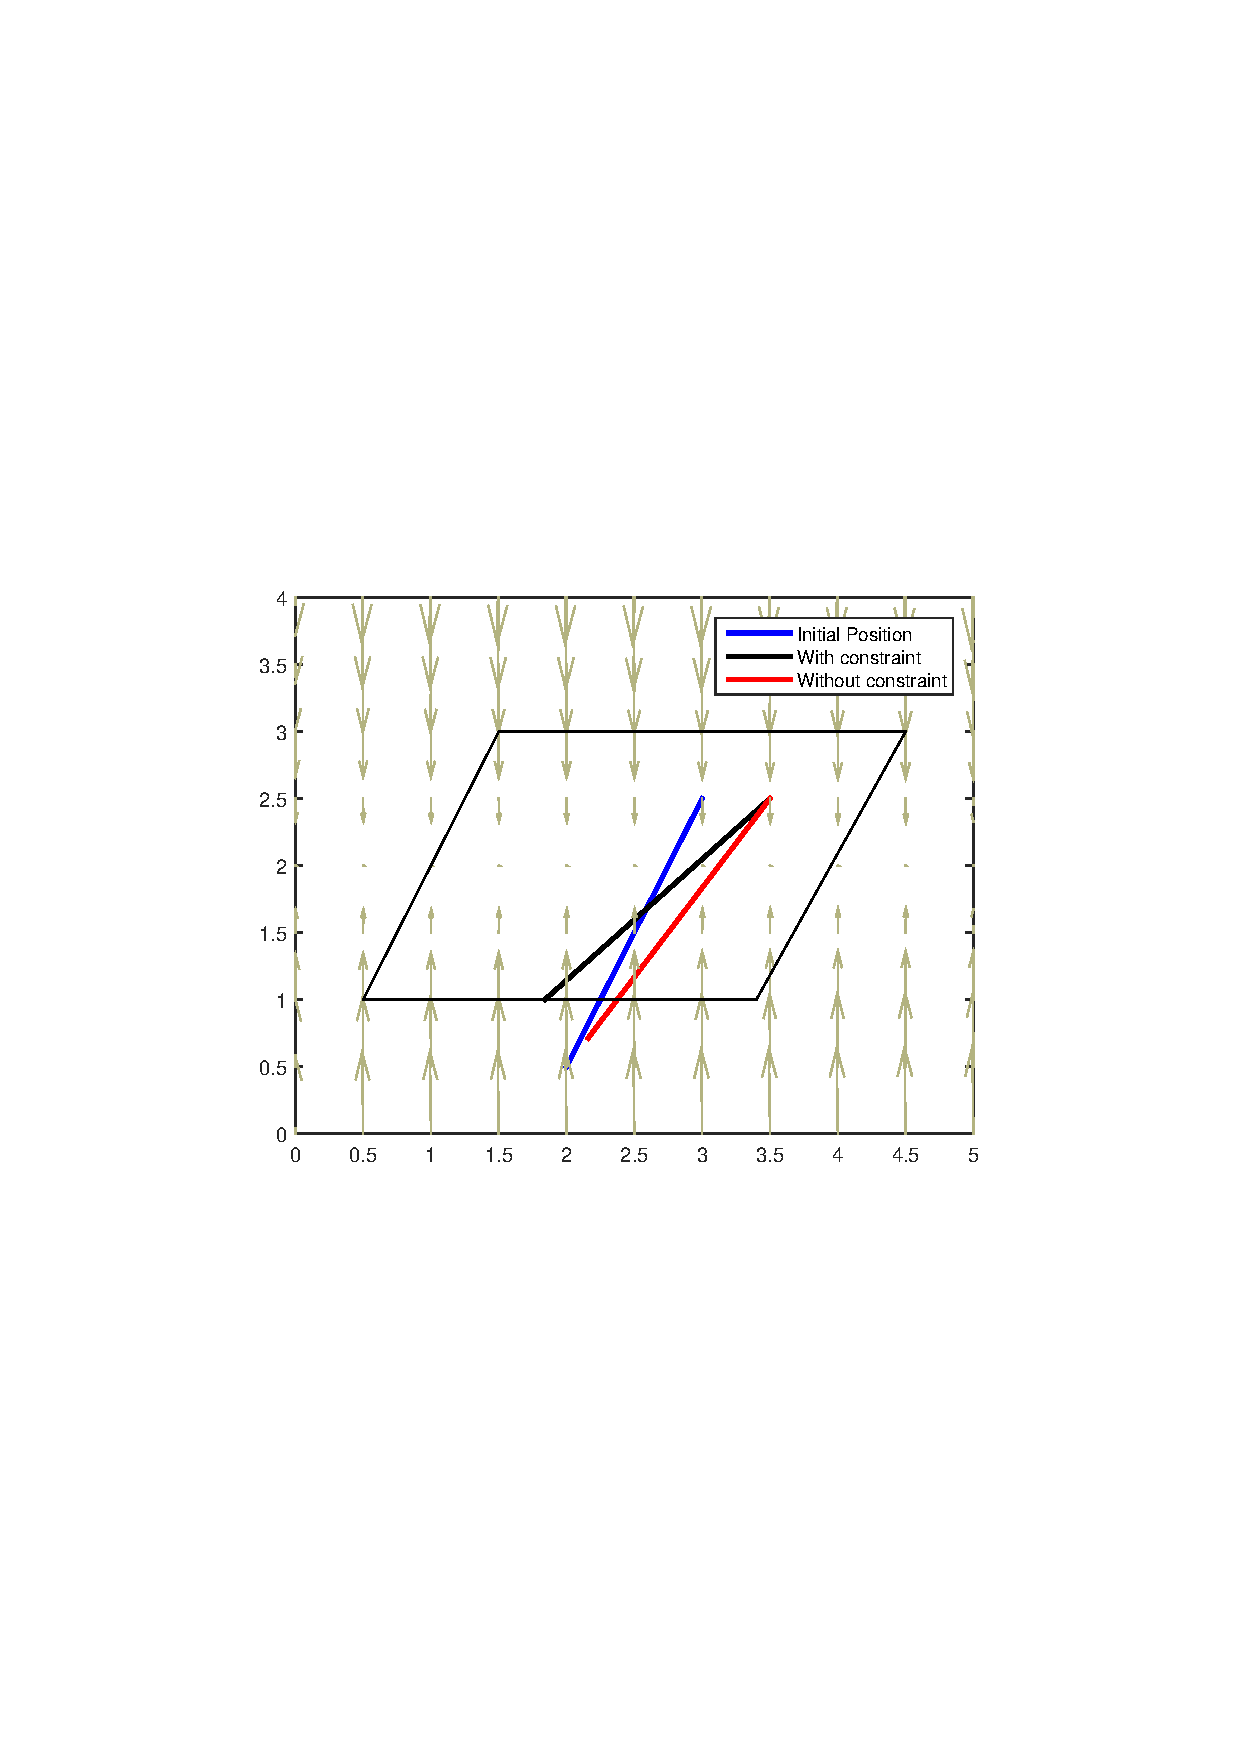
\includegraphics[scale=0.5]{figures/fig10b.pdf}
\caption{ Effect of gradient of inequality constraint in pulling the tail into the quadrilateral duct \label{fig:quadgradient}}
\end{figure}


\subsection{Representation of duct using two non-intersecting continuous curves}
If the non-intersecting border curves of the duct can be analytically expressed, then the equation of the surface patch will simply be,
\begin{align}
\mathbf{x}_i(u,v)= \zeta_1(u)\left(1-{v}\right) +\zeta_2(u)\left({v}\right)
\end{align}
For example, [fig11] shows a 2D duct defined by two curves $\zeta_1(u) = \left[u,~\sin\left(u \right)\right]^T$ and $\zeta_2(u) = \left[u,~\sin\left(u +\frac{\pi}{8}\right)+1\right]^T$ and a path chosen midway between the two curves. The equation of the surface generated by this curves will be

\begin{figure}[ht!]
    \centering
    \begin{subfigure}{0.48\textwidth}
        \centering
        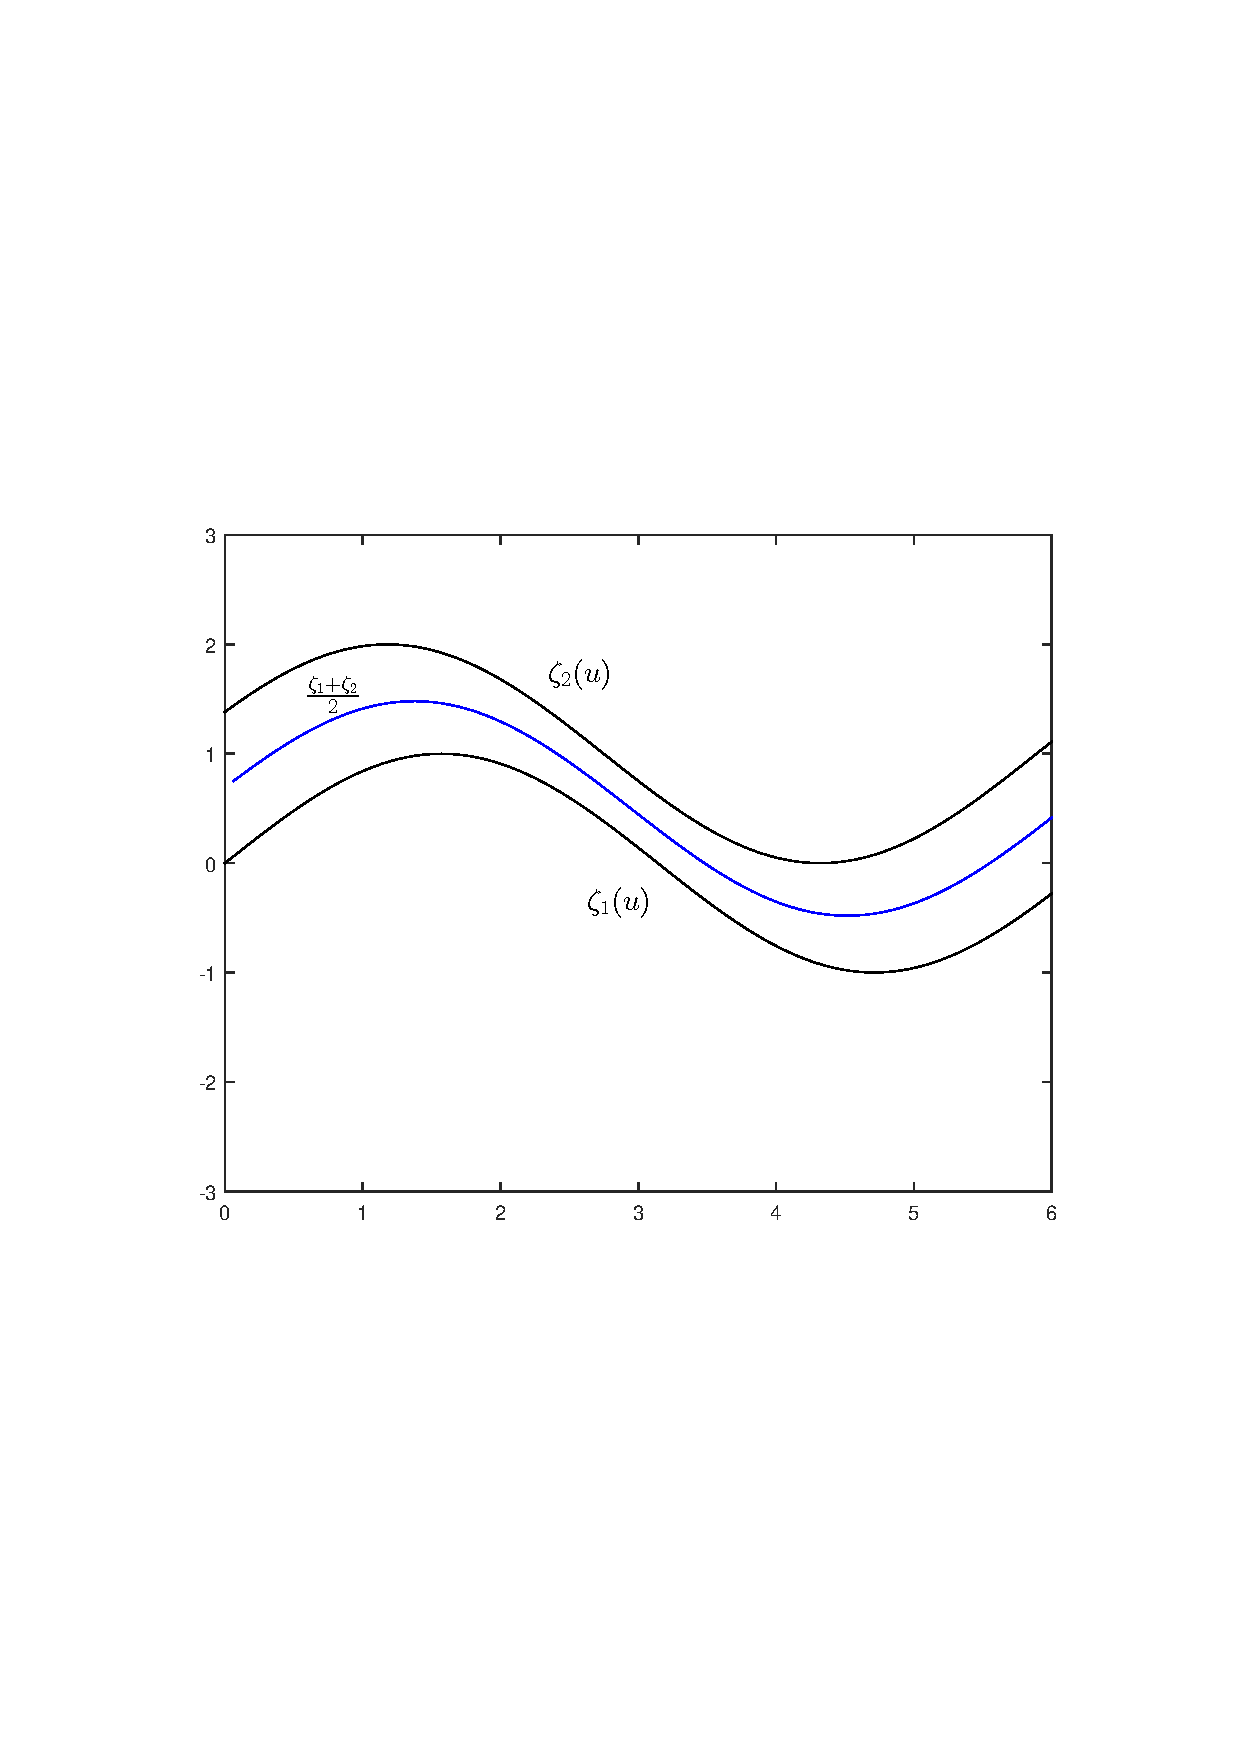
\includegraphics[width=0.75\linewidth]{figures/fig11.pdf}
        \caption{Example of analytical duct \label{fig:analyticduct}}
    \end{subfigure}%
    \begin{subfigure}{0.48\textwidth}
        \centering
        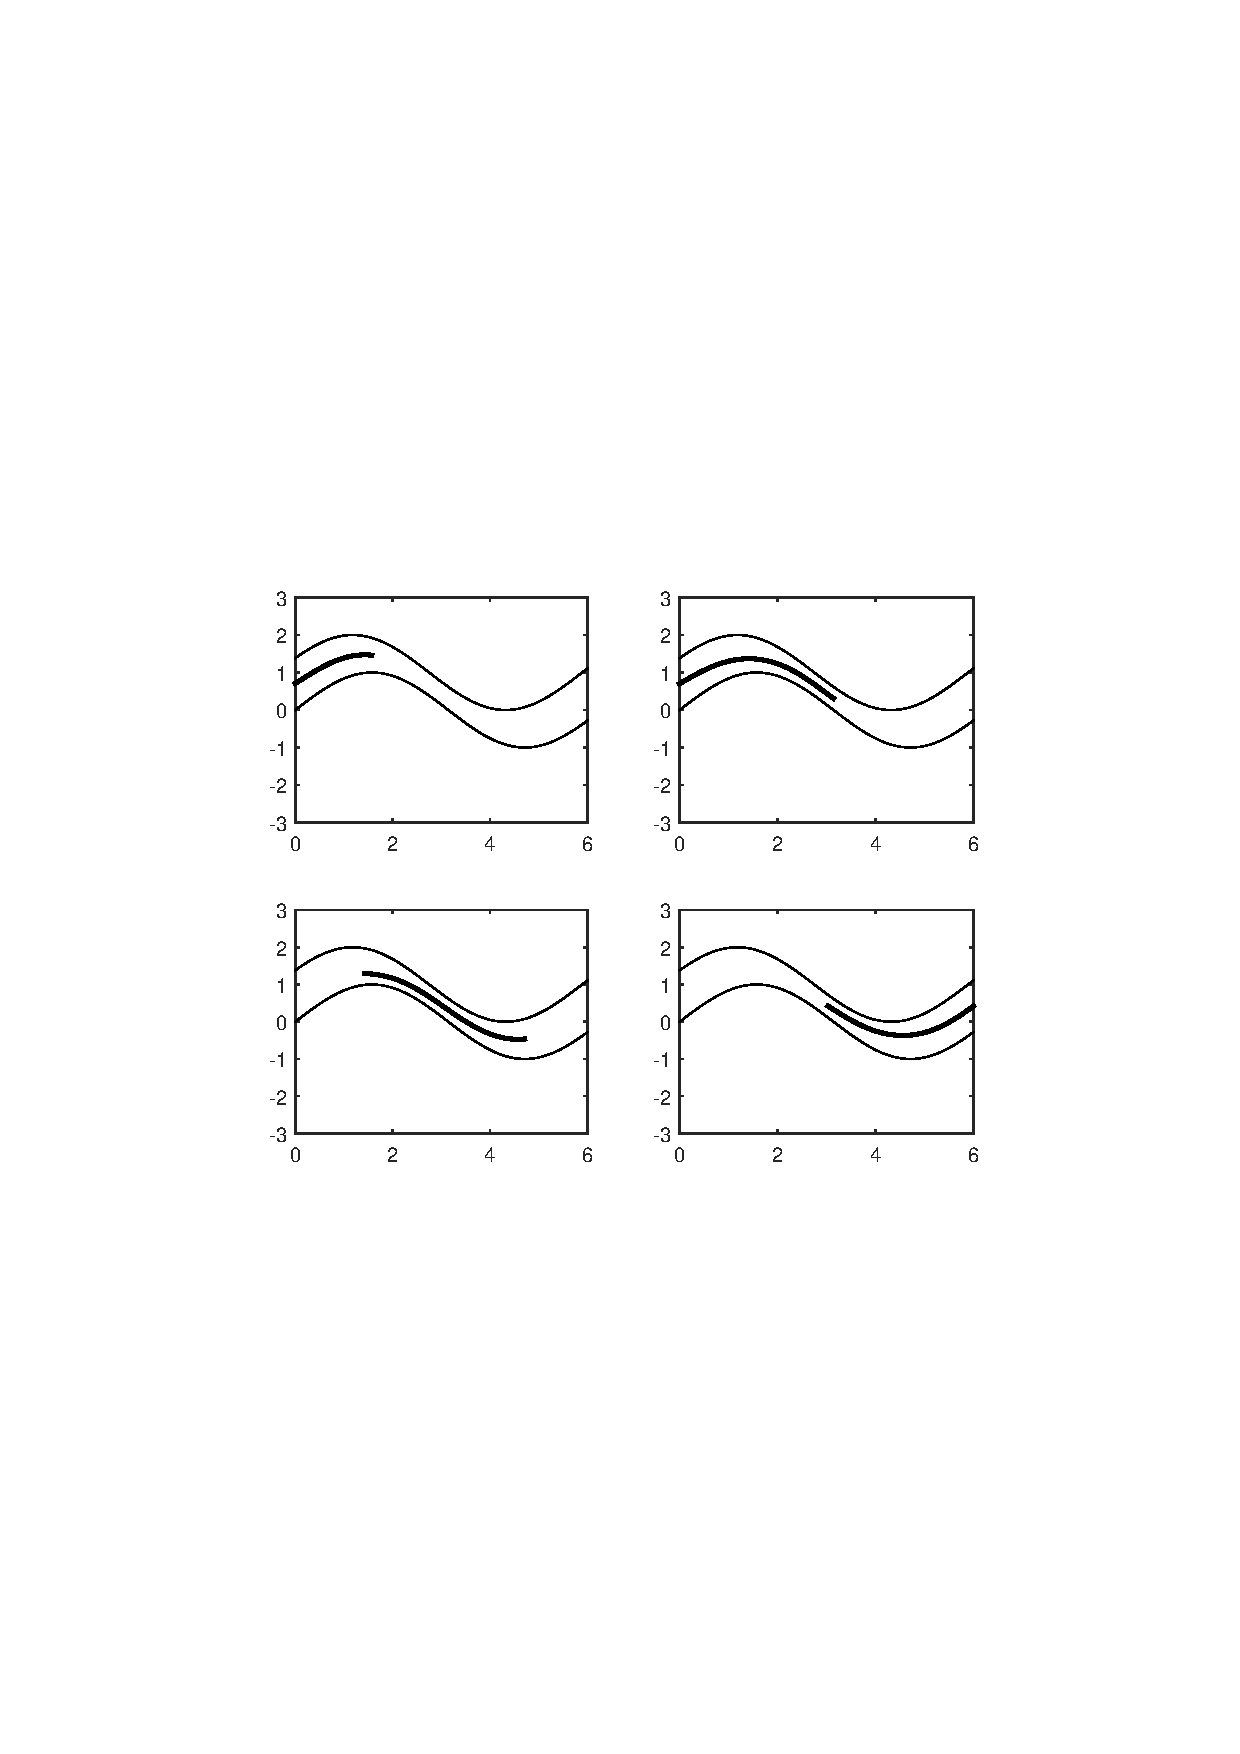
\includegraphics[width=0.75\linewidth]{figures/fig12.pdf}
        \caption{Motion through analytical duct \label{fig:analyticductmotion}}
    \end{subfigure}
    \caption{ Tractrix based algorithm on analytical duct}
\end{figure}


\begin{align}
\begin{bmatrix}
x(u,v)\\y(u,v)
\end{bmatrix} = 
\begin{bmatrix}
u\\\sin\left(u\right)+\left[\sin\left(u+\frac{\pi}{8}\right)-\sin\left(u\right)+1 \right]v
\end{bmatrix}
\end{align}
which has the analytical solution for $u$ and $v$:
\begin{align*}
u &= x\\
v &= \frac{y-\sin\left(x\right)}{\sin\left(x+\frac{\pi}{8}\right)-\sin\left(x\right)+1}
\end{align*}
In this case, we will solve the equations:
\begin{align}
\label{eq:analy2D}
\min_{\textbf{x}_t} &\Vert \textbf{x}_t-\textbf{X}_t \Vert\\
\nonumber \text{sub:~~~} &\Vert \textbf{x}_h - \textbf{x}_t \Vert -L_0 = 0\\
&0< v\vert_{\mathbf{x}_t}< 1
\end{align} 
 An example movement of hyper-redundant manipulator through the duct is shown in [fig12]. However, analytical solution is not always viable for complex equations and numerical procedure must be employed to find the values of $u$ and $v$ corresponding to the given tail point to be classified. The equation to be used is \ref{eq:minx,u,v}.




\section{Motion planning through 3D ducts}
In this section, we will explain a few methods to represent ducts in 3D and how motion planning is achieved in the same.
\subsection{Representation of duct using combination of super-ellipsoids}
In Cartesian co-ordinate system in $R^3$, the surface of a super-ellipsoid follows the equation:
\begin{equation}
f(x,y,z) : \left[ \left\lbrace \left(\frac{x}{a} \right)^{\frac 2e} +\left(\frac{y}{b} \right)^{\frac 2e} \right\rbrace^{\frac{e}{n}} +\left(\frac{z}{c} \right)^{\frac 2n}  \right]^\frac n2-1 =0
\end{equation}


By changing the parameters $a,b,c$ and $n$, we get different closed surfaces as shown in [fig13]. By combining different super-ellipse shapes, we can generate a 3D duct as shown in [fig14]

[fig13] : What are super-ellipsoids.
[fig14] : Duct represented by super-ellipsoids.

The procedure to calculate the inside-outside condition is same as that of the method described in section [ref sec]. The final equations will be same as [\ref{eq: min,mingx}]. An example problem with duct approximated using super-ellipsoids is shown in [fig15]. As mentioned in the case for super-ellipses, solution to the path planning problem with ducts represented by super-ellipsoids is fast as explained in section ??. Identifying the shapes which fit the duct, is also same as the method mentioned in section ??.

[fig15] : Motion through super-ellipsoid ducts


\subsection{Representation of duct as a set of connected cylinders}
Another more involved method in representing duct is by series of connected cylinders. By linearly interpolating two circles in 3D, we get the parametric equation of surface of the cylinder as (refer Appendix for the detailed expressions):
\begin{align}
\label{eq:cylinder}
x = C_1(u,t,\theta),~~y = C_2(u,t,\theta),~~z = C_3(u,t,\theta)
\end{align}
where the parameters $u,t$ and $\theta$ varies along the radial, axial and circumferential direction of the cylinder respectively (refer [fig16]). Similar to the representation in [sec], $0\leq u< 1$ and $0<t<1$ classifies the point as inside the cylinder. The final minimization problem is same as that of [\ref{eq:min,u,v,im}]. One major advantage of using this formulation is that by changing the radius of cylinder from $r$ to $r-\delta$, we can easily implement a clearance of $\delta$ units from the walls of the cylinder. Motion of link chain through the duct connected using cylinders is shown in [fig17]

[fig16] : Connected cylinder forming duct
[fig17] : Motion of HR manipulator through connected-cylinders duct


\subsection{Representation of duct as point clouds}
Most practically convenient way of representing the duct would be as the a collection of point clouds  ($\mathbf{R}_i,i=1,2,...,N$ where $N$ is the number of points in the cloud) such as obtained from Stereolithographic formatted file (STL). It is possible to pose the optimization problem in the form:
\begin{align}
\label{eq:STLeqs}
\min_{\textbf{x}_t} &\Vert \textbf{x}_t-\textbf{X}_t \Vert\\
\nonumber \text{sub:~~~} &\Vert \textbf{x}_h - \textbf{x}_t \Vert -L_0 = 0\\
&[\mathbf{A}]\mathbf{x}_t+\mathbf{B}\leq 0
\end{align}
where $\mathbf{A}$ is a $m\times 3$ matrix and $\mathbf{B}$ is a $m\times 1$ vector. The left hand side of $m$ inequalities represent the equations of $m$ number of planes spanned by three adjacent points in the cloud. The $i^\text{th}$ equation, $A_{i}^1x_t+A_{i}^2y_t+A_{i}^3z_t+B_i$ takes a value less than zero when the point $\mathbf{x}_t$ is in the half space which contains the origin and is greater than zero otherwise. The value also provides the attractive gradient which will ensure that the point stays inside the duct. However, in actual implementation, this procedure will be tedious and for practical convenience, it is possible to classify the point $\mathbf{x}_t$ as inside or outside the hull using the algorithm proposed by ??. The attracting gradient which ensures the point to be inside the duct--as the case with the previous methods-- can be provided using the artificial potential field generated from the centroid of the point cloud in conjunction with the output of the in-out function. The inequality constraint then becomes
\begin{align}
\label{eq:STLineq}
w(\mathbf{R})\frac{1}{\Vert(\overline{\mathbf{R}})-\mathbf{x}_t\Vert}\leq 0
\end{align}
where $w(\overline{\mathbf{R}})$ represents the output from in-out function which is either 1 for the point being outside and 0 for the point being inside the cloud or on the bounding surface\footnote{Unlike the previous classification problems, the bounding surface will also be considered as inside the surface in this case.}. 

Another interesting prospect of this method is its application in obstacle avoidance where the left hand side of the equation \Cref{eq:STLineq} will be greater than zero. The obstacle avoidance methods which follow the equation given by \Cref{eq:obstacle_avoidance_opt} is often limited to shapes which can be modelled analytically. Though the algorithm shown here is limited to convex shapes, they can be applied to more complex and non-symmetric shapes.

\subsection{Analytical ducts}
As mentioned in the section??, it is possible to express a few class of ducts using closed form expressions. For example, the helical duct shown in [fig ??] can be expressed using the equations
\begin{align}
\begin{bmatrix}
x(u,\theta,\phi)\\y(u,\theta,\phi)\\z(u,\theta,\phi)
\end{bmatrix} = 
\begin{bmatrix}
\left(R+ru\cos\theta \right)\cos\phi\\
\left(R+ru\cos\theta \right)\sin\phi\\
\left(R+r\sin\theta \right)+H\phi
\end{bmatrix}
\end{align}

where $R,r,H$ are the radius of the helix, half the thickness of duct and the height of the helix respectively. The solution method involves solving the equation:
\begin{align}
\label{eq:analy2D}
\min_{\textbf{x}_t} &\Vert \textbf{x}_t-\textbf{X}_t \Vert\\
\nonumber \text{sub:~~~} &\Vert \textbf{x}_h - \textbf{x}_t \Vert -L_0 = 0\\
&0\leq u < 1
\end{align} 
There exists multiple solutions to this equation and one has to conditionally check the validity of the solution while implementation. The motion of hyper-redundant robot through a helical duct is shown in fig??.

\section{Examples and discussion}
In this section, we present two practical examples of the above mentioned methods and some discussion  on the implementation of the same.
\subsection{Examples of motion planning through ducts}
\subsubsection{Motion planning through a GI tract}
There has been a growing interest in simulating motion of endoscope through GI tract for developing simulators for endoscopy and for implementing path planning for endoscopic and laparoscopic surgical robots. In this section, we simulate the natural motion of an endoscope through GI tract. For simulation, we use the stereolithographic data of GI tract obtained from ??. We have demonstrated both the methods presented in [sec] and [sec] for approximating the GI tract. In the first method, a collection of points are manually selected from the STL file where super-elliposids are fit based on least square error minimization techniques. Representation of GI tract as series of super-ellipsoids is shown in [fig19]

[fig19] : Representation of GI tract as super-ellipsoids.

For representing GI tract as cylinders, we first found out the medial axis of the duct using ??. Then at equal intervals of distance along the medial axis, planes are drawn normal to the same. The collection of points which are in the close proximity of the plane are selected and a circle is fitted on the points using least square error minimization. The parameters so obtained are used for the cylinder equations in [\ref{eq:cylinder}]. Representation of GI tract as a series of connected cylinders is shown in [fig20]

[fig20] : Representation of GI tract as cylinders.

The realistic motion simulation of endoscope through GI tract is shown in [fig21]

[fig21] : Motion through GI tract
\subsubsection{Motion planning for search and rescue operations}
Exploring obstacle-cluttered environments such as in an earthquake hit zone is one of the major applications that necessitates the use of hyper-redundant manipulators. In this example, we show how the proposed algorithms can be effectively used in such applications. With reference to [fig ??], the objective of the hyper-redundant manipulator, consisting of 20 links is to 1) enter the scene through the hole in the outer wall, 2) Pass through the vent to get inside the room, 3) Explore the objects 1,2 and 3 located inside the blue hull and 4) Exit without colliding with the complex shapes given by objects 4 and 5. Here, the exploration problem is effectively tackled using the following constraints added to the optimization problem (refer Fig ??): 1) An ellipsoid of the size of the hole located in the outer wall 2) collection of cylindrical ducts to represent the vent, 3) STL models for the objects 1,2 and 3 and 4) Ellipsoid at the last bend in the path to avoid collision with the complex shapes of objects 4 and 5. It is easy to verify that the existing geometry based motion planning of robot will be quite complicated for this scene while using the methods proposed in this paper, the problem can be addressed with only 6 constraints. The six constraints in this case are actively selected so that they become activate only when the position of the head is in the vicinity of the objects/ shapes. Figure [??] shown the simulated results for the motion of manipulator along a chosen path. 

\subsection{Computational complexity and limitations of tractrix based scheme}

... for now the procedure takes ?? takes to compute. We plan to reduce this in the future.
Another limitation of tractrix based scheme proposed is the locking of a link which traverses sharp bends for non-differentiable ducts given by representations proposed in ?? and ??, as shown in [fig ??]. Here, the expected subsequent position of the link is the one which bends around the corner following the head, while the tractrix based approach will result in the link being pulled downwards (like bicycle chain on sprocket) to the position 2 shown in the figure, which is the theoretical minimum for the optimization problem satisfying the constraints. Hence, the bending angle at the corners in the most general case may be limited to $90^\circ$. In order to avoid this issue, the sharp corners may be blunted off by adding extra points in the corners as shown in [fig ??]. For the curve $\zeta_1$ which includes a corner represented by the points $\mathbf{P}_1,\mathbf{P}_2$ and $\mathbf{P}_3$, and a given link length $L_0$ such that $\Vert \mathbf{P}_1-\mathbf{P}_2\Vert\geq L_0$  and $\Vert \mathbf{P}_3-\mathbf{P}_2\Vert\geq L_0$, the curvature may be increased by adding another line segment so that the final points be $\mathbf{P}_1,\mathbf{P}_2^a,\mathbf{P}_2^b,\mathbf{P}_3$  where the point $\mathbf{P}_2^a=\mathbf{P}_2+\frac{L_0}{\Vert \mathbf{P}_2-\mathbf{P}_1}\Vert\left(\mathbf{P}_1-\mathbf{P}_2\Vert\right)$ and $\mathbf{P}_2^b$ may be obtained form solving the equations
\begin{align}
\Vert \mathbf{P}_2-\mathbf{P}_2^b\Vert = L_0,~~\Vert \mathbf{P}_2^a-\mathbf{P}_2^b\Vert = L_0
\end{align} 
Needless to say, this rounding off is subject to practical feasibility.



\subsection{Tractrix  emulates natural motion}
Motion simulated using the approach discussed in this paper imparts realism due to the minimal movement of tail with respect to the head. In nature this effect is created due to the friction or other resistive forces acting in the lateral direction of the link. In the absence of friction, displacement given in the head will result in a simple translation of link. In other words, $\mathbf{x}_t$ in this case, will be same as $\mathbf{x}_h$. In figure [fig22], we can see the effect of friction on a connected link chain which is pulled in one direction. The discrepancy between natural movement and the simulation based on the tractrix approach is because tractrix represents the ideal scenario with motion of tail limited only in the direction of motion of the link due to very high friction while in natural motion, there is always some degree of translation possible. This slippage could be included in the formulation, however, by adding a slip vector to the tail displacement. Since the slippage amounts to the translation of link in the direction of link, slip vector will be in the direction of head displacement and can be written as as $\mathbf{s} = \nu \mathbf{X}_h$, where $\nu<1$ is a constant. $\nu=0$ represents the ideal tractrix case with friction and $\nu=1$ represents pure translation of the link. Including this vector, the minimization function may be written as:
\begin{align}
\min_{\textbf{x}_t} &\Vert \textbf{x}_t-\left(\mathbf{X}_t + \nu \mathbf{X}_h \right) \Vert
\end{align}

[fig22] : Experiments using bicycle chain

Using a constant value of $\nu = ??$, we can see from [fig23] that the formulation conforms with the actual final pose with good accuracy. 

[fig23] : Tractrix with $\nu$.


\section{Conclusions}

??


\subsection{Contributions and scope of future work}
uses LAPACK and heavy solvers.. not really required. instead a stripped version of the interior point will do quite well for fast near real-time implementation. 

\section{Appendix}	\crefalias{section}{appsec}
\subsection{Analytical expressions for $u,v$ for quadrilateral patch}\label{app:Analylit_u_v_quad}
\begin{align}
&\quad {v} = \frac{k_1-k_2\pm \sqrt{\left(k_2-k_1\right)^2-4k_3k_4}}{2k_3},~~{u} = \frac{\left(x-{}^xP_{i-1}+{v}\right)}{\left( a_2+{v} a_3 \right)}\\
\nonumber\text{ where, }k_1 &= \left(b_1b_2+b_0b_3 \right),~~k_2 = \left(a_1a_2+a_0a_3 \right),~~
k_3 = \left(a_1a_3-b_1b_3 \right),~~k_4=\left(a_0a_2-b_0b_2 \right)\\
\nonumber a_0 &= y-{}^yP_{i-1},~a_1 = {}^yP_{i-1}-{}^yP_i,~a_2 = {}^xQ_{i-1}-{}^xP_{i-1},~a_3 = \left({}^xQ_{i}-{}^xP_i\right)-\left({}^xQ_{i-1}-{}^xP_{i-1}\right)\\
\nonumber b_0 &= x-{}^xP_{i-1},~b_1 = {}^xP_{i-1}-{}^xP_i,~b_2 = {}^yQ_{i-1}-{}^yP_{i-1},~b_3 = \left({}^yQ_{i}-{}^yP_i\right)-\left({}^yQ_{i-1}-{}^yP_{i-1}\right)
\end{align}

If ${}^xP_{i-1}={}^xP_{i}$ and ${}^xQ_{i-1}={}^xQ_{i}$, 
\begin{align}
{u} = \frac{b_0}{a_2},~~{v} = \frac{a_0a_2-\left(a_3+a_2 \right)}{a_1\left(b_0-a_2\right)+b_0\left(b_3-b_2 \right)}
\end{align}

\subsection{Parametric equation of solid cylinder}\label{app:parametric_u_v_solid_cyl}
\begin{align}
x & = C_1(u,t,\theta)=\left(r_1m_1u\cos\theta +m_2 \right)\left(1-t \right)+\left(r_2n_1u\cos\theta+n_2 \right)t\\
y & = C_2(u,t,\theta)=\left(r_1m_3u\cos\theta +r_1m_4u\sin\theta +m_5 \right)\left(1-t \right)+\left(r_2n_3u\cos\theta+r_2n_4u\sin\theta+n_5 \right)t\\
z & = C_3(u,t,\theta)=\left(r_1m_6u\cos\theta +r_1m_7u\sin\theta +m_8 \right)\left(1-t \right)+\left(r_2n_6u\cos\theta+r_2n_7u\sin\theta+n_8 \right)t
\end{align}
where
\begin{align*}
m_1 = \cos{}^1\phi_2,~m_2 = {}^1x_c,~m_3 = \sin{}^1\phi_1\sin{}^1\phi_2,~m_4=\cos{}^1\phi_1, \nonumber \\
m_5 = {}^1y_c,~m_6=-\cos{}^1\phi_1\sin{}^1\phi_2,~m_7=\sin{}^1\phi_1,~m_8={}^1z_c \nonumber
\end{align*}
and
\begin{align*}
n_1 = \cos{}^2\phi_2,~n_2 = {}^2x_c,~n_3 = \sin{}^2\phi_1\sin{}^2\phi_2,~n_4=\cos{}^2\phi_1, \nonumber \\
n_5 = {}^2y_c,~n_6=-\cos{}^2\phi_1\sin{}^2\phi_2,~n_7=\sin{}^2\phi_1,~n_8={}^2z_c \nonumber
\end{align*}
The quantity ${}^1\left(\cdot\right)$ and ${}^2\left(\cdot\right)$ represent the corresponding parameters of the circles at the ends of the cylinder. $\phi_1$ and $\phi_2$ are the angles about the Y and X-axes which the plane of the circle is rotated, $(x_c,y_c,z_c)$ is the co-ordinate of the center of the circle.

\subsection{An algorithm for classifying a point with respect to a polyhedron}\label{app:polyhedron_point}
\indent Classification a point with respect to a triangulated domain is a very well known problem and many methods exist, which offer various advantages in terms of computational complexities. In the algorithm \cref{alg:in_hull}, we describe a method, to classify a given set of points $O$ with respect to $\mathcal{S}$ as inside ($O_{in}$) and outside ($O_{out}$). Our algorithm and it's Matlab implementation\footnote{We have used a Matlab function inhull.m, a fully vectorized implementation of the algorithm, made available by John D'Errico for free usage. } is not very efficient at higher dimensions but seems to perform reasonably well at 3D, by taking less than 8 seconds to classify about 10,000 points with respect to a meshed domain. 
\begin{algorithm}[ht!]
	\textbf{Purpose :} To classify a set of points $ O $ with respect to $\partial \mathcal{S}$\\
	\KwIn{The set $ O $, $O\in \Re^3$ and $O \equiv O_{in}\cup O_{out}$ }
	\KwOut{$ O_{in},~ O_{out}$}
	\begin{algorithmic}[1]
		\STATE Obtain the $\alpha$ shape $\mathcal{S}$ of the set of points $\mathbb{S}$
		\STATE Obtain $C$, the center of $\mathcal{S}$ by taking the mean of the vertices of the $N$ facets constituting $\partial \mathcal{S}$
		\FOR {$i=1,2,...,N$}
		\STATE Calculate the normal to the $i^{th}$ facet, $A_n^i=(f_i^1-f_i^2)\times(f_i^2-f_i^3)$
		\STATE Choose a point $A^i$ on the $i^{th}$ facet and move $A_n^i$ to $A^i$
		\STATE Ensure that $A_n^i$ is directed inside, towards $C$
		\STATE $H(i)=\langle\vec{O_i-A_i}, A_n^i\rangle$
		\ENDFOR 
		\IF {$H(i)\geq 0 ~\forall i$}
		\STATE Classify $O_1 \in O_{in}$ as inside, otherwise classify $O_1\in O_{out}$  		\ENDIF
	\end{algorithmic}
	
	\caption{Algorithm for classifying points as inside ($O_{in}$) or outside ($O_{out}$) of a triangulated domain}		
	\label{alg:in_hull}
\end{algorithm}

%\bibliography{journalref}


\begin{thebibliography}{99}

We have to see IEEE reference format.
%%1
%\bibitem{Gaylord1958}
%R.~H. Gaylord (1958), 
%\newblock ``Fluid actuated motor system and stroking device'',
%\newblock {\em US Patent  2,844,126} (July~22 1958).
%
%%2
%\bibitem{Joseph1960}
%L.~Joseph (1960), 
%newblock ``Artificial muscle'', 
%\newblock {\em Life} {\bf 14}, pp. 87--88.
%
%%3
%\bibitem{Pillsbury2015}
%T.~E. Pillsbury, C.~S. Kothera, N.~M. Wereley (2015),
%\newblock `` Effect of bladder wall thickness  on miniature pneumatic artificial muscle performance'', 
%\newblock{\em Bioinspiration \& Biomimetics}, {\bf 10}~(5), pp. 055006.


\end{thebibliography}


\end{document}